\documentclass{beamer}\usepackage[]{graphicx}\usepackage[]{color}
%% maxwidth is the original width if it is less than linewidth
%% otherwise use linewidth (to make sure the graphics do not exceed the margin)
\makeatletter
\def\maxwidth{ %
  \ifdim\Gin@nat@width>\linewidth
    \linewidth
  \else
    \Gin@nat@width
  \fi
}
\makeatother

\definecolor{fgcolor}{rgb}{0, 0, 0}
\newcommand{\hlnum}[1]{\textcolor[rgb]{0.533,0,0.133}{#1}}%
\newcommand{\hlstr}[1]{\textcolor[rgb]{0.667,0.267,0}{#1}}%
\newcommand{\hlcom}[1]{\textcolor[rgb]{1,0.533,0}{#1}}%
\newcommand{\hlopt}[1]{\textcolor[rgb]{0,0,0}{\textbf{#1}}}%
\newcommand{\hlstd}[1]{\textcolor[rgb]{0,0,0}{#1}}%
\newcommand{\hlkwa}[1]{\textcolor[rgb]{0.4,0.067,0.067}{\textbf{#1}}}%
\newcommand{\hlkwb}[1]{\textcolor[rgb]{0,0,0.4}{\textbf{#1}}}%
\newcommand{\hlkwc}[1]{\textcolor[rgb]{0,0,0.4}{#1}}%
\newcommand{\hlkwd}[1]{\textcolor[rgb]{0,0.267,0.4}{#1}}%
\let\hlipl\hlkwb

\usepackage{framed}
\makeatletter
\newenvironment{kframe}{%
 \def\at@end@of@kframe{}%
 \ifinner\ifhmode%
  \def\at@end@of@kframe{\end{minipage}}%
  \begin{minipage}{\columnwidth}%
 \fi\fi%
 \def\FrameCommand##1{\hskip\@totalleftmargin \hskip-\fboxsep
 \colorbox{shadecolor}{##1}\hskip-\fboxsep
     % There is no \\@totalrightmargin, so:
     \hskip-\linewidth \hskip-\@totalleftmargin \hskip\columnwidth}%
 \MakeFramed {\advance\hsize-\width
   \@totalleftmargin\z@ \linewidth\hsize
   \@setminipage}}%
 {\par\unskip\endMakeFramed%
 \at@end@of@kframe}
\makeatother

\definecolor{shadecolor}{rgb}{.97, .97, .97}
\definecolor{messagecolor}{rgb}{0, 0, 0}
\definecolor{warningcolor}{rgb}{1, 0, 1}
\definecolor{errorcolor}{rgb}{1, 0, 0}
\newenvironment{knitrout}{}{} % an empty environment to be redefined in TeX

\usepackage{alltt}
\newenvironment{changemargin}[2]{%
\begin{list}{}{%
\setlength{\topsep}{0pt}%
\setlength{\leftmargin}{#1}%
\setlength{\rightmargin}{#2}%
\setlength{\listparindent}{\parindent}%
\setlength{\itemindent}{\parindent}%
\setlength{\parsep}{\parskip}%
}%
\item[]}{\end{list}}
\usepackage{graphicx}
\usepackage{amsmath}
\usepackage{url}
\usetheme{Madrid}
\usecolortheme{beaver}
\setbeamertemplate{navigation symbols}{}
\titlegraphic{
\includegraphics[width=5cm]{..//..//S-DS-VC-RGB.png}}
%\logo{
\includegraphics[width=0.1\textwidth,keepaspectratio]{..//..//UOACrest.png}}
\author[SCC]{Statistical Consulting Centre}%\\
\institute[\href{mailto:consulting@stat.auckland.ac.nz}
  {consulting@stat.auckland.ac.nz}]{\href{mailto:consulting@stat.auckland.ac.nz}
  {consulting@stat.auckland.ac.nz}\\
%Statistical Consulting Centre\\
The Department of Statistics\\
The University of Auckland}
\title[Session 5 -- Graphics]{NZSSN Courses: Introduction to \texttt{R}}
\subtitle{Session 5 -- Graphics}
\date{2 March, 2017}
\IfFileExists{upquote.sty}{\usepackage{upquote}}{}
\begin{document}
%\SweaveOpts{concordance=TRUE}
\maketitle

\begin{frame}[fragile]
  \frametitle{Exploring your data}

\begin{itemize}
  \item Examine for patterns, relationships, structures, and
    other features.
  \item Do this using graphs, tables and summary statistics.
  \item Patterns are more easily seen in graphs.
  \item Remember:
    \begin{center}
      ``\texttt{R} is a free software environment for statistical computing and \emph{graphics}''
    \end{center}
\end{itemize}
\end{frame}


\begin{frame}
  \frametitle{Designing graphs}
Two important considerations when designing a graph:
\vspace{0.5cm}
\begin{itemize}
\item It should have something to say.
  \begin{itemize}
  \item Decide what information you want your graph to display.
  \item Graphical software is capable of producing any number of different graphs, so generating graphs with meaningless information is quite simple to do!
  \end{itemize}
\item It should be easy to interpret.
  \begin{itemize}
  \item Simplicity is key!
  \item Sufficiently large fonts, all axes labelled, clearly defined legends, etc.
  \end{itemize}
\end{itemize}
\end{frame}

\begin{frame}[fragile]
  \frametitle{Some functions for drawing graphs}
  \begin{itemize}
  \item Usually, we use \texttt{plot()} to create a graph and then
    \texttt{lines()}, \texttt{points()}, \texttt{text()}, and other
    commands to annotate it.
  \item \texttt{plot()} does appropriate things for different types of
    variables (see later examples).
  \item Variables of type \texttt{cha}racter are not suitable for plotting (and analysis). Convert such variables to type \texttt{factor}.
  \item There are no ``erase'' or ``undo'' functions, so store your commands in an \texttt{R} script.
  \end{itemize}
\end{frame}


\begin{frame}[fragile]
  \frametitle{Boxplots}
\begin{knitrout}
\definecolor{shadecolor}{rgb}{0.965, 0.965, 0.965}\color{fgcolor}\begin{kframe}
\begin{alltt}
\hlkwd{with}\hlstd{(issp.df,} \hlkwd{plot}\hlstd{(age.group, total.lik))}
\end{alltt}
\end{kframe}
\end{knitrout}

\begin{figure}[h]
  \vspace{-20pt}
  \centering
  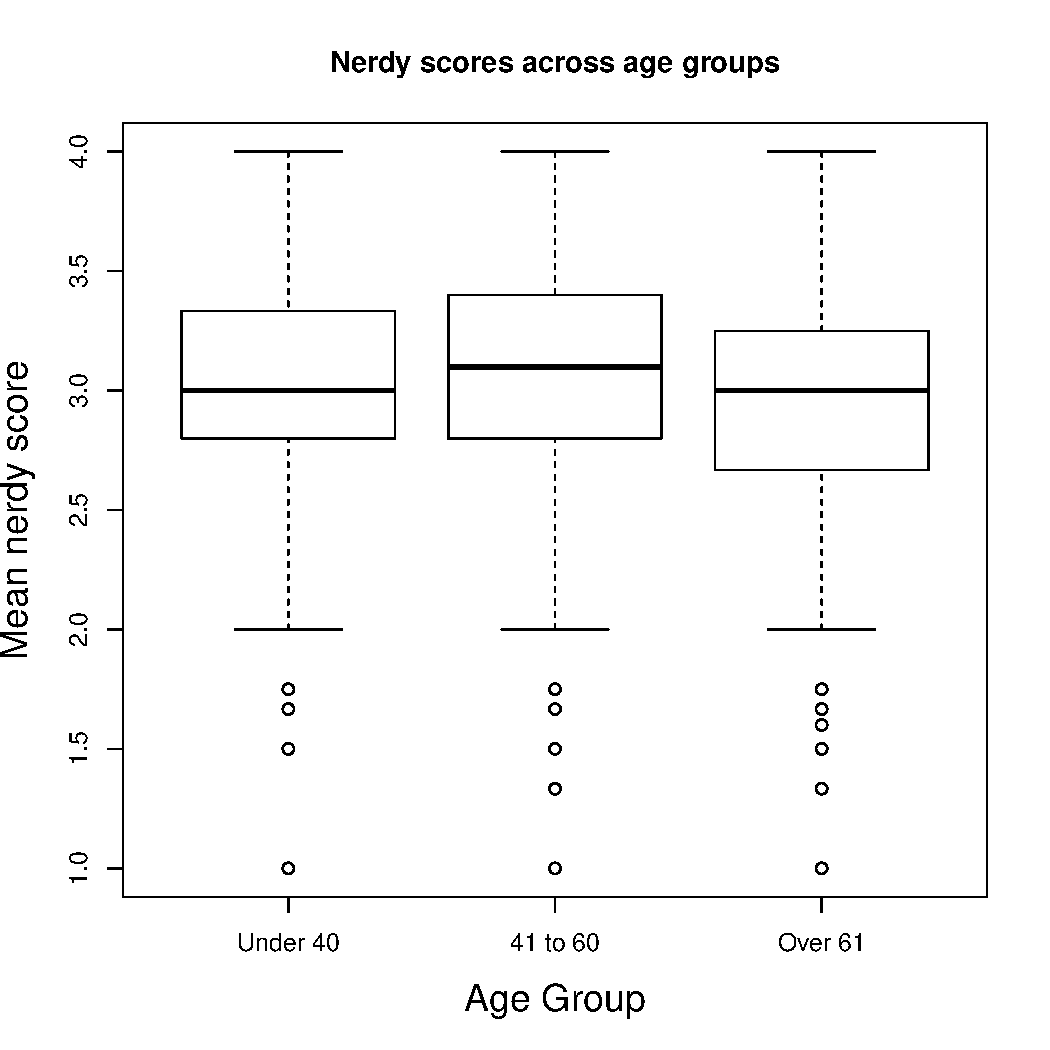
\includegraphics[height = 0.6\textwidth, keepaspectratio]{Figure/box1}
  %\vspace{-20pt}
  %\caption{Boxplots of PM10 in 2006--2012}
  \label{fig:box1}
\end{figure}
\end{frame}


\begin{frame}[fragile]
  \frametitle{Boxplots}
\begin{knitrout}
\definecolor{shadecolor}{rgb}{0.965, 0.965, 0.965}\color{fgcolor}\begin{kframe}
\begin{alltt}
\hlkwd{with}\hlstd{(issp.df,} \hlkwd{plot}\hlstd{(Gender, total.lik))}
\end{alltt}


{\ttfamily\noindent\color{warningcolor}{Warning in xy.coords(x, y, xlabel, ylabel, log): NAs introduced by coercion}}

{\ttfamily\noindent\color{warningcolor}{Warning in min(x): no non-missing arguments to min; returning Inf}}

{\ttfamily\noindent\color{warningcolor}{Warning in max(x): no non-missing arguments to max; returning -Inf}}

{\ttfamily\noindent\bfseries\color{errorcolor}{Error in plot.window(...): need finite 'xlim' values}}\end{kframe}

\includegraphics[width=\maxwidth]{figure/unnamed-chunk-3-1} 

\end{knitrout}
\end{frame}

\begin{frame}[fragile]
  \frametitle{Boxplots}
\texttt{age.group} is a factor but \texttt{Gender} is not.
\begin{knitrout}
\definecolor{shadecolor}{rgb}{0.965, 0.965, 0.965}\color{fgcolor}\begin{kframe}
\begin{alltt}
\hlkwd{class}\hlstd{(issp.df}\hlopt{$}\hlstd{Gender)}
\end{alltt}
\begin{verbatim}
[1] "character"
\end{verbatim}
\begin{alltt}
\hlkwd{class}\hlstd{(issp.df}\hlopt{$}\hlstd{age.group)}
\end{alltt}
\begin{verbatim}
[1] "factor"
\end{verbatim}
\end{kframe}
\end{knitrout}
\end{frame}

\begin{frame}[fragile]
  \frametitle{Boxplots}

\begin{knitrout}
\definecolor{shadecolor}{rgb}{0.965, 0.965, 0.965}\color{fgcolor}\begin{kframe}
\begin{alltt}
\hlkwd{with}\hlstd{(issp.df,} \hlkwd{plot}\hlstd{(}\hlkwd{factor}\hlstd{(Gender), total.lik))}
\end{alltt}
\end{kframe}

{\centering 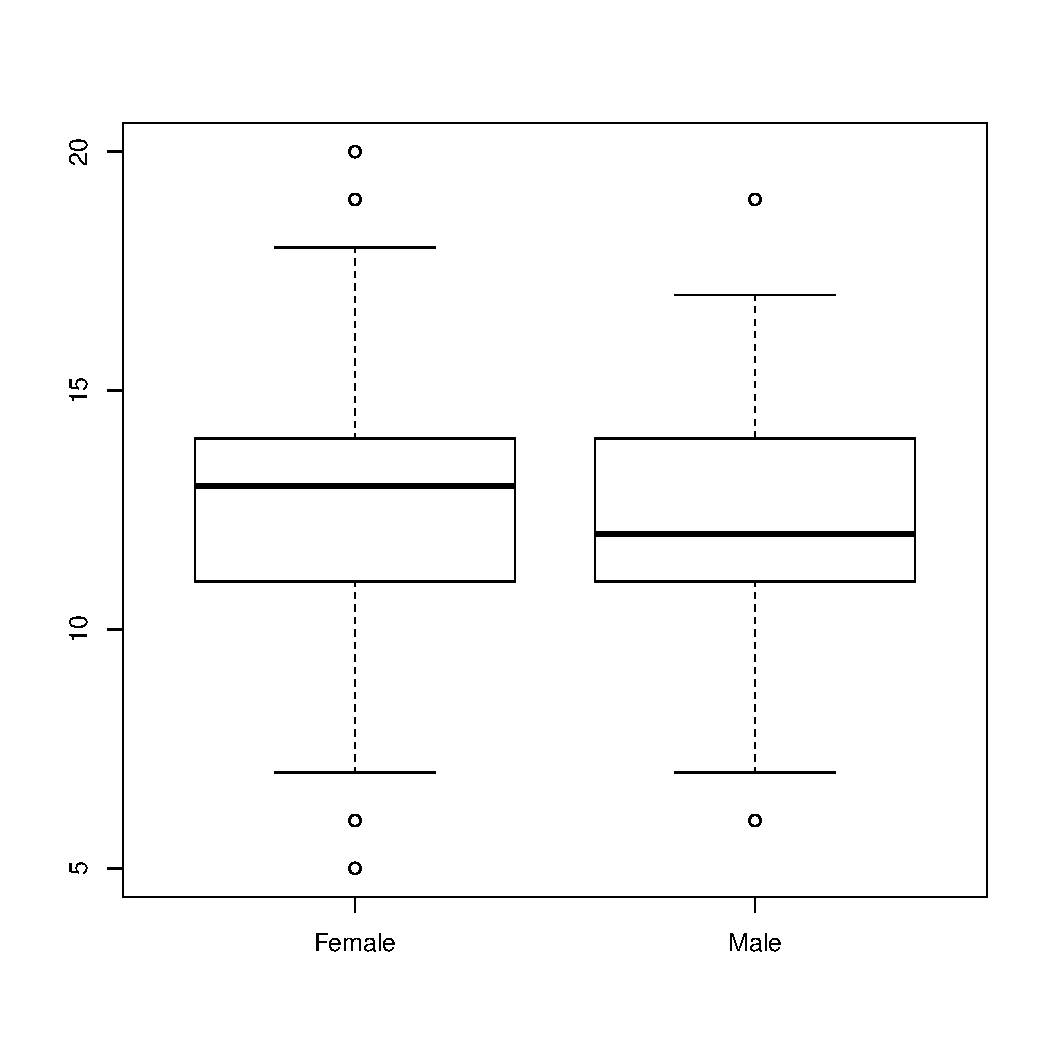
\includegraphics[width=0.6\linewidth]{figure/box2-1} 

}



\end{knitrout}
\end{frame}



\begin{frame}[fragile]
  \frametitle{Axes need labels}
\begin{knitrout}
\definecolor{shadecolor}{rgb}{0.965, 0.965, 0.965}\color{fgcolor}\begin{kframe}
\begin{alltt}
\hlkwd{with}\hlstd{(issp.df,} \hlkwd{plot}\hlstd{(age.group, total.lik,}
    \hlkwc{xlab} \hlstd{=} \hlstr{"Age Group"}\hlstd{,} \hlkwc{ylab} \hlstd{=} \hlstr{"Total score"}\hlstd{))}
\end{alltt}
\end{kframe}
\end{knitrout}

\begin{figure}[h]
  \vspace{-25pt}
  \centering
  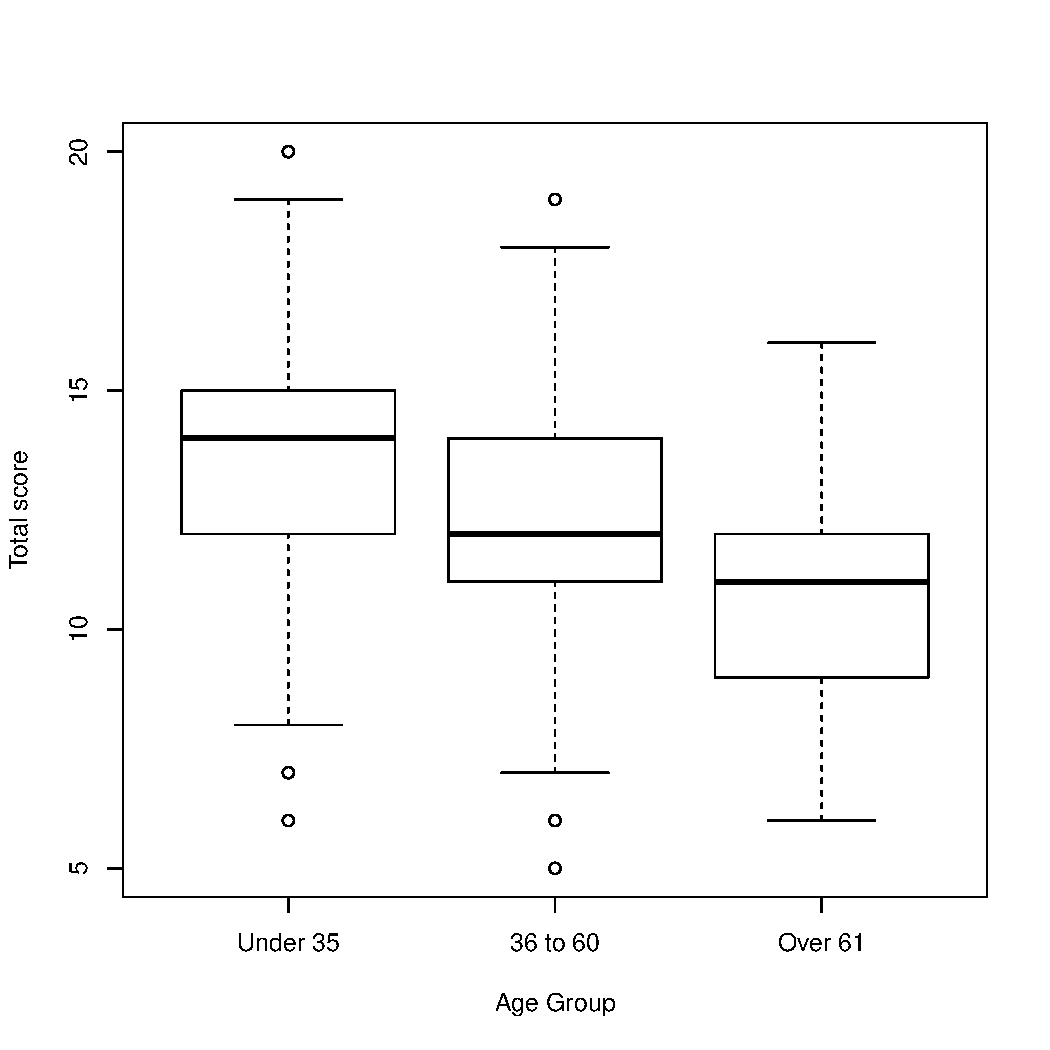
\includegraphics[height = 0.6\textwidth, keepaspectratio]{Figure/box3}
  \label{fig:box3}
\end{figure}
\end{frame}

\begin{frame}[fragile]
  \frametitle{Axis labels are too small!!}
\begin{knitrout}
\definecolor{shadecolor}{rgb}{0.965, 0.965, 0.965}\color{fgcolor}\begin{kframe}
\begin{alltt}
\hlkwd{with}\hlstd{(issp.df,} \hlkwd{plot}\hlstd{(age.group, total.lik,} \hlkwc{cex.lab} \hlstd{=} \hlnum{1.5}\hlstd{,}
    \hlkwc{xlab} \hlstd{=} \hlstr{"Age Group"}\hlstd{,} \hlkwc{ylab} \hlstd{=} \hlstr{"Total score"}\hlstd{))}
\end{alltt}
\end{kframe}
\end{knitrout}

\begin{figure}[h]
  \vspace{-25pt}
  \centering
  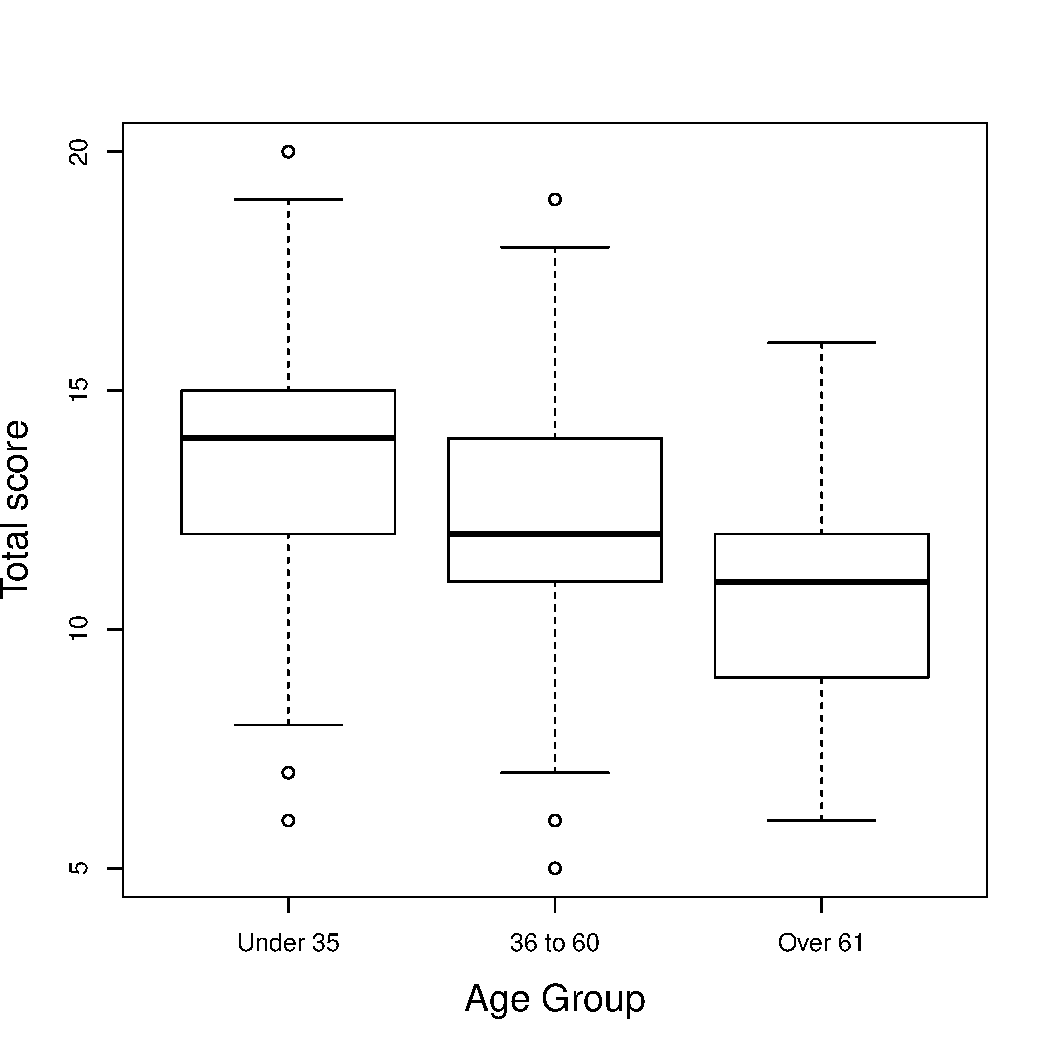
\includegraphics[height = 0.6\textwidth, keepaspectratio]{Figure/box4}
  \label{fig:box4}
\end{figure}
\end{frame}

\begin{frame}[fragile]
  \frametitle{Sometimes you need a title}
\begin{knitrout}
\definecolor{shadecolor}{rgb}{0.965, 0.965, 0.965}\color{fgcolor}\begin{kframe}
\begin{alltt}
\hlkwd{with}\hlstd{(issp.df,} \hlkwd{plot}\hlstd{(age.group, total.lik,} \hlkwc{cex.lab} \hlstd{=} \hlnum{1.5}\hlstd{,}
   \hlkwc{xlab} \hlstd{=} \hlstr{"Age Group"}\hlstd{,} \hlkwc{ylab} \hlstd{=} \hlstr{"Total score"}\hlstd{,}
    \hlkwc{main} \hlstd{=} \hlstr{"Total Score versus Age"}\hlstd{))}
\end{alltt}
\end{kframe}
\end{knitrout}

\begin{figure}[h]
  \vspace{-20pt}
\centering
  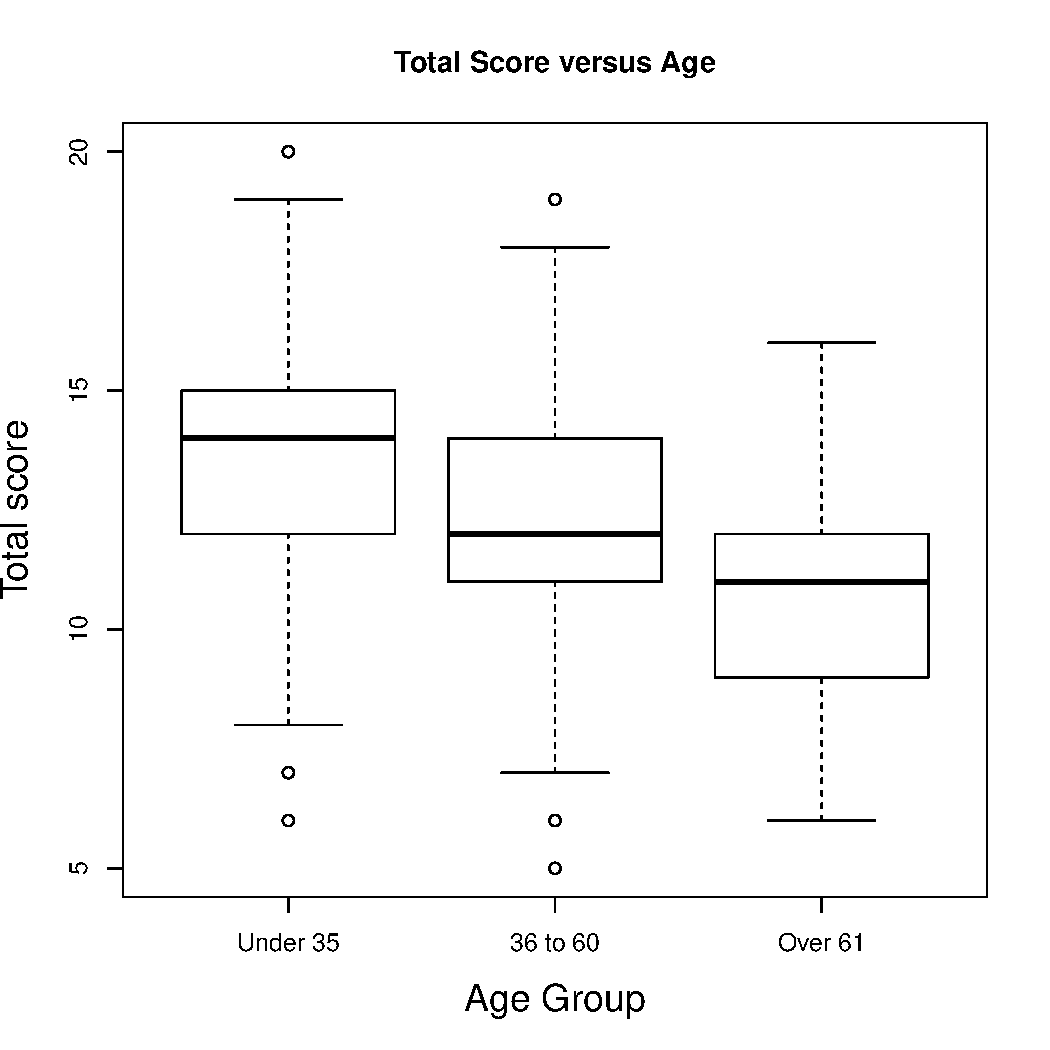
\includegraphics[height = 0.55\textwidth, keepaspectratio]{Figure/box5}
 \label{fig:box5}
\end{figure}
\end{frame}

\begin{frame}[fragile]
  \frametitle{\texttt{boxplot()}}
More flexible than \texttt{plot()}, \textbf{if} drawing boxplots. Check the help documentation for more details.
\begin{knitrout}
\definecolor{shadecolor}{rgb}{0.965, 0.965, 0.965}\color{fgcolor}\begin{kframe}
\begin{alltt}
\hlkwd{with}\hlstd{(issp.df,} \hlkwd{boxplot}\hlstd{(total.lik}\hlopt{~}\hlstd{age.group,}
   \hlkwc{xlab} \hlstd{=} \hlstr{"Age Group"}\hlstd{,} \hlkwc{ylab} \hlstd{=} \hlstr{"Total score"}\hlstd{))}
\end{alltt}
\end{kframe}
\end{knitrout}

\begin{figure}[h]
  \vspace{-20pt}
\centering
  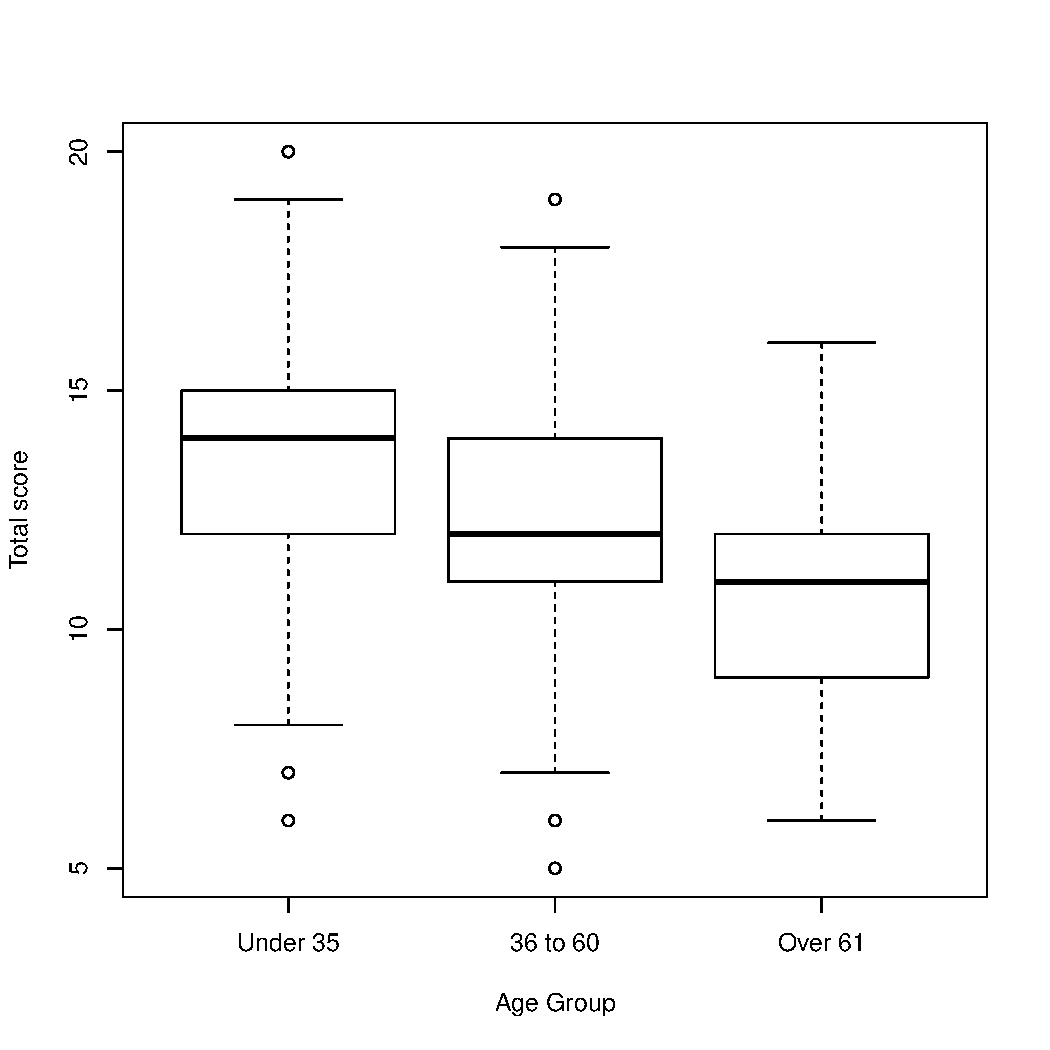
\includegraphics[height = 0.5\textwidth, keepaspectratio]{Figure/box6}
 \label{fig:box6}
\end{figure}
\end{frame}

\begin{frame}[fragile]
  \frametitle{Importance of childhood obedience by age group}
  Q5: Is obedience important in terms of preparing children for life?\\
  \vspace{2mm}
  Examine the data via a two-way frequency table.
  \vspace{-2mm}
\begin{knitrout}
\definecolor{shadecolor}{rgb}{0.965, 0.965, 0.965}\color{fgcolor}\begin{kframe}
\begin{alltt}
\hlkwd{with}\hlstd{(issp.df,} \hlkwd{table}\hlstd{(Q5, age.group))}
\end{alltt}
\end{kframe}
\end{knitrout}
\vspace{-6mm}
\begin{knitrout}
\definecolor{shadecolor}{rgb}{0.965, 0.965, 0.965}\color{fgcolor}\begin{kframe}
\begin{verbatim}
                  age.group
Q5                 Under 35 36 to 60 Over 61
  be obedient            38       74      75
  can t choose, dk       30       34      12
  NA, refused             6        9       9
  think themselves      259      353     122
\end{verbatim}
\end{kframe}
\end{knitrout}
\vspace{-5mm}
\begin{knitrout}
\definecolor{shadecolor}{rgb}{0.965, 0.965, 0.965}\color{fgcolor}\begin{kframe}
\begin{alltt}
\hlstd{issp.df}\hlopt{$}\hlstd{Q5} \hlkwb{<-} \hlkwd{with}\hlstd{(issp.df,}
                \hlkwd{ifelse}\hlstd{(Q5} \hlopt{==} \hlstr{"can t choose, dk"} \hlopt{|}
                       \hlstd{Q5} \hlopt{==} \hlstr{"NA, refused"}\hlstd{,} \hlnum{NA}\hlstd{, Q5))}
\end{alltt}
\end{kframe}
\end{knitrout}
\end{frame}

\begin{frame}[fragile]
  \frametitle{Importance of childhood obedience by age group}
First, convert counts to percentages. Why?
\begin{knitrout}
\definecolor{shadecolor}{rgb}{0.965, 0.965, 0.965}\color{fgcolor}\begin{kframe}
\begin{alltt}
\hlstd{q5.age} \hlkwb{<-} \hlkwd{with}\hlstd{(issp.df,}
               \hlnum{100}\hlopt{*}\hlkwd{prop.table}\hlstd{(}\hlkwd{table}\hlstd{(Q5, age.group),} \hlnum{2}\hlstd{))}
\hlkwd{round}\hlstd{(q5.age,} \hlnum{1}\hlstd{)}
\end{alltt}
\begin{verbatim}
                  age.group
Q5                 Under 35 36 to 60 Over 61
  be obedient          12.8     17.3    38.1
  think themselves     87.2     82.7    61.9
\end{verbatim}
\end{kframe}
\end{knitrout}
How do we graphically display the information contained in this table?
\end{frame}

\begin{frame}[fragile]
  \frametitle{Absolute disaster!!!}
\begin{knitrout}
\definecolor{shadecolor}{rgb}{0.965, 0.965, 0.965}\color{fgcolor}\begin{kframe}
\begin{alltt}
\hlkwd{barplot}\hlstd{(q5.age,} \hlkwc{xlab} \hlstd{=} \hlstr{"Age group in years"}\hlstd{,}
        \hlkwc{ylab} \hlstd{=} \hlstr{"Percentage"}\hlstd{)}
\end{alltt}
\end{kframe}

{\centering 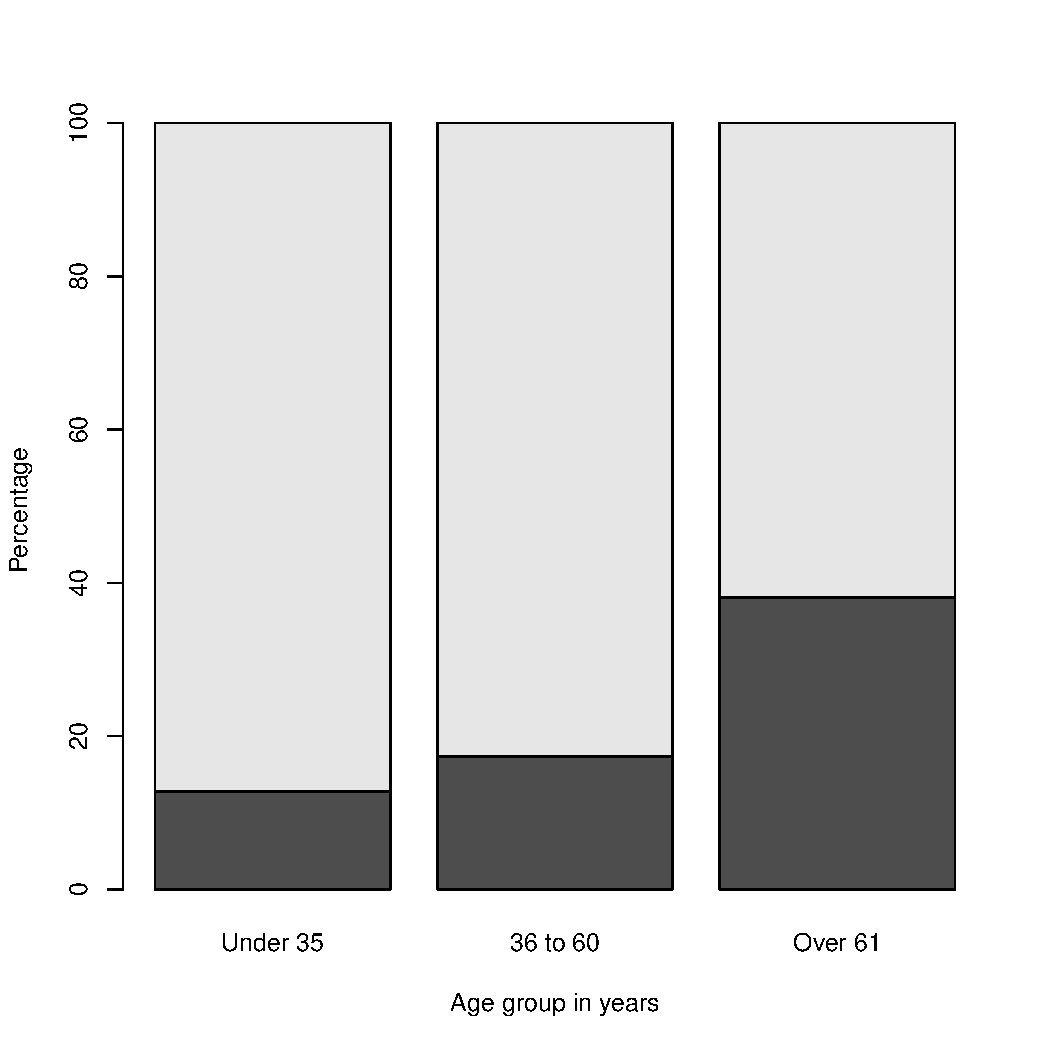
\includegraphics[width=0.45\linewidth]{figure/bar1-1} 

}



\end{knitrout}
\end{frame}

\begin{frame}[fragile]
  \frametitle{Better}
\begin{knitrout}
\definecolor{shadecolor}{rgb}{0.965, 0.965, 0.965}\color{fgcolor}\begin{kframe}
\begin{alltt}
\hlkwd{barplot}\hlstd{(q5.age,} \hlkwc{beside} \hlstd{=} \hlnum{TRUE}\hlstd{,} \hlkwc{ylab} \hlstd{=} \hlstr{"Percentage"}\hlstd{,}
        \hlkwc{xlab} \hlstd{=} \hlstr{"Age group in years"}\hlstd{)}
\end{alltt}
\end{kframe}

{\centering 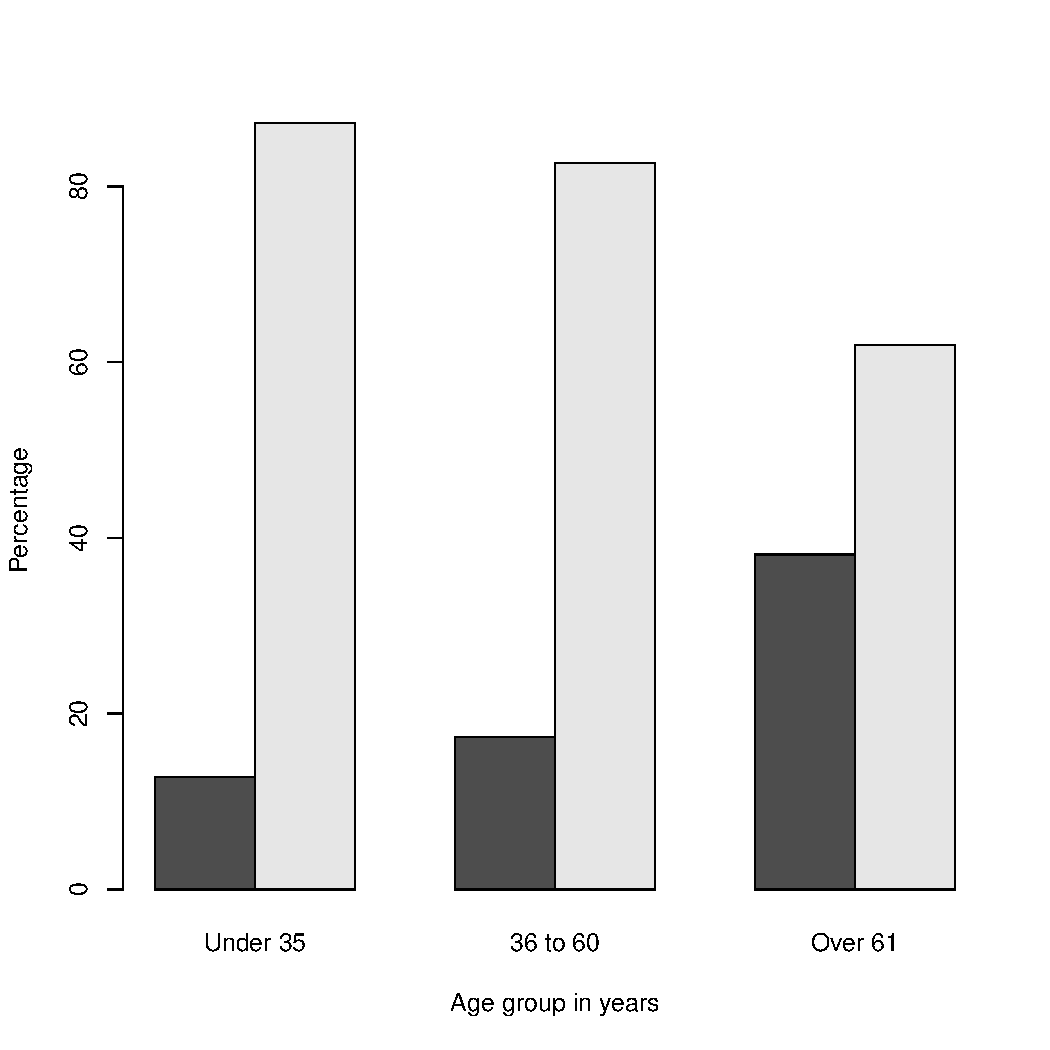
\includegraphics[width=0.45\linewidth]{figure/bar2-1} 

}



\end{knitrout}
\end{frame}

\begin{frame}[fragile]
  \frametitle{Line along horizontal axis?}
\begin{knitrout}
\definecolor{shadecolor}{rgb}{0.965, 0.965, 0.965}\color{fgcolor}\begin{kframe}
\begin{alltt}
\hlkwd{barplot}\hlstd{(q5.age,} \hlkwc{beside} \hlstd{=} \hlnum{TRUE}\hlstd{,} \hlkwc{ylab} \hlstd{=} \hlstr{"Percentage"}\hlstd{,}
        \hlkwc{xlab} \hlstd{=} \hlstr{"Age group in years"}\hlstd{)}
\hlkwd{abline}\hlstd{(}\hlkwc{h} \hlstd{=} \hlnum{0}\hlstd{)}
\end{alltt}
\end{kframe}

{\centering 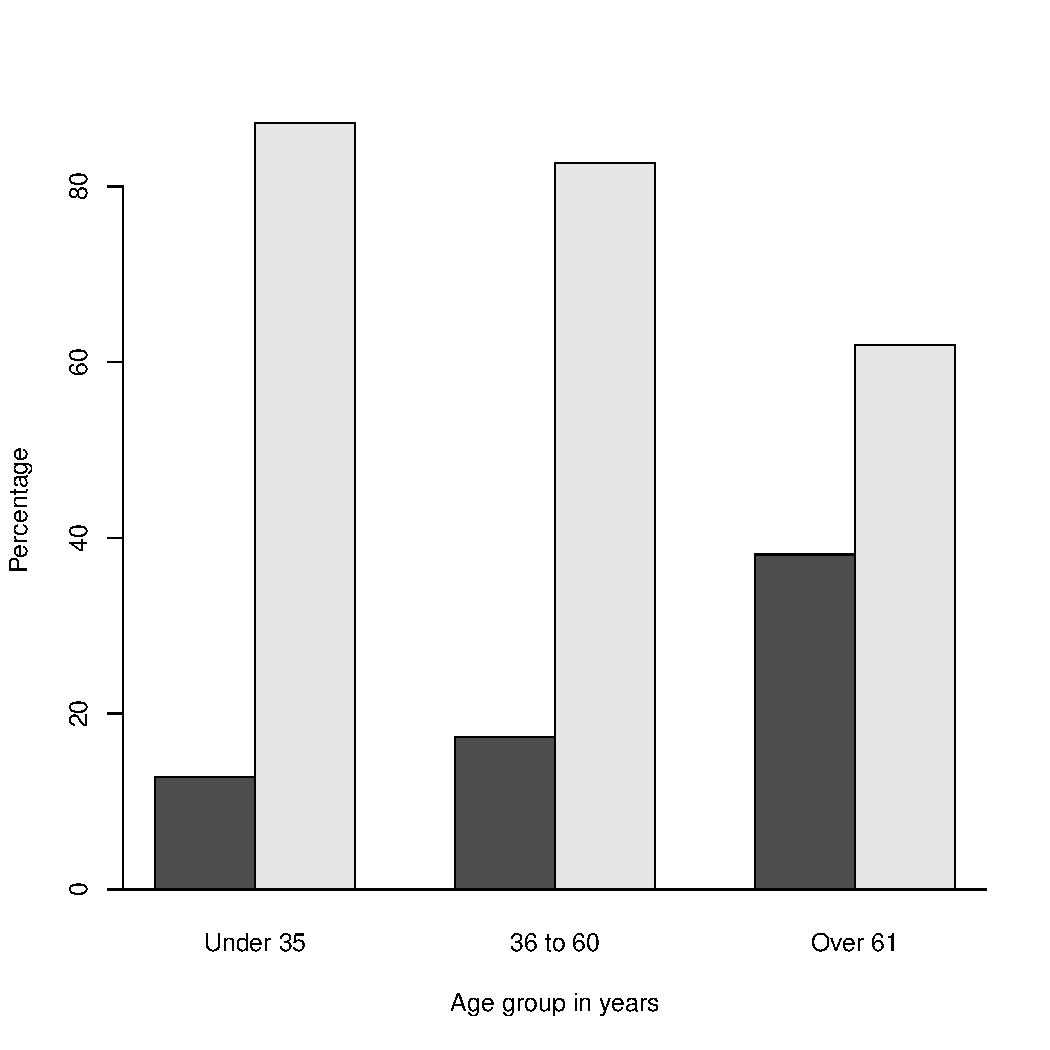
\includegraphics[width=0.45\linewidth]{figure/bar10-1} 

}



\end{knitrout}
\end{frame}

\begin{frame}[fragile]
  \frametitle{Vertical axis higher than bars?}
\begin{knitrout}
\definecolor{shadecolor}{rgb}{0.965, 0.965, 0.965}\color{fgcolor}\begin{kframe}
\begin{alltt}
\hlkwd{barplot}\hlstd{(q5.age,} \hlkwc{beside} \hlstd{=} \hlnum{TRUE}\hlstd{,} \hlkwc{ylab} \hlstd{=} \hlstr{"Percentage"}\hlstd{,}
        \hlkwc{xlab} \hlstd{=} \hlstr{"Age group in years"}\hlstd{,} \hlkwc{ylim} \hlstd{=} \hlkwd{c}\hlstd{(}\hlnum{0}\hlstd{,} \hlnum{100}\hlstd{))}
\hlkwd{abline}\hlstd{(}\hlkwc{h} \hlstd{=} \hlnum{0}\hlstd{)}
\end{alltt}
\end{kframe}

{\centering 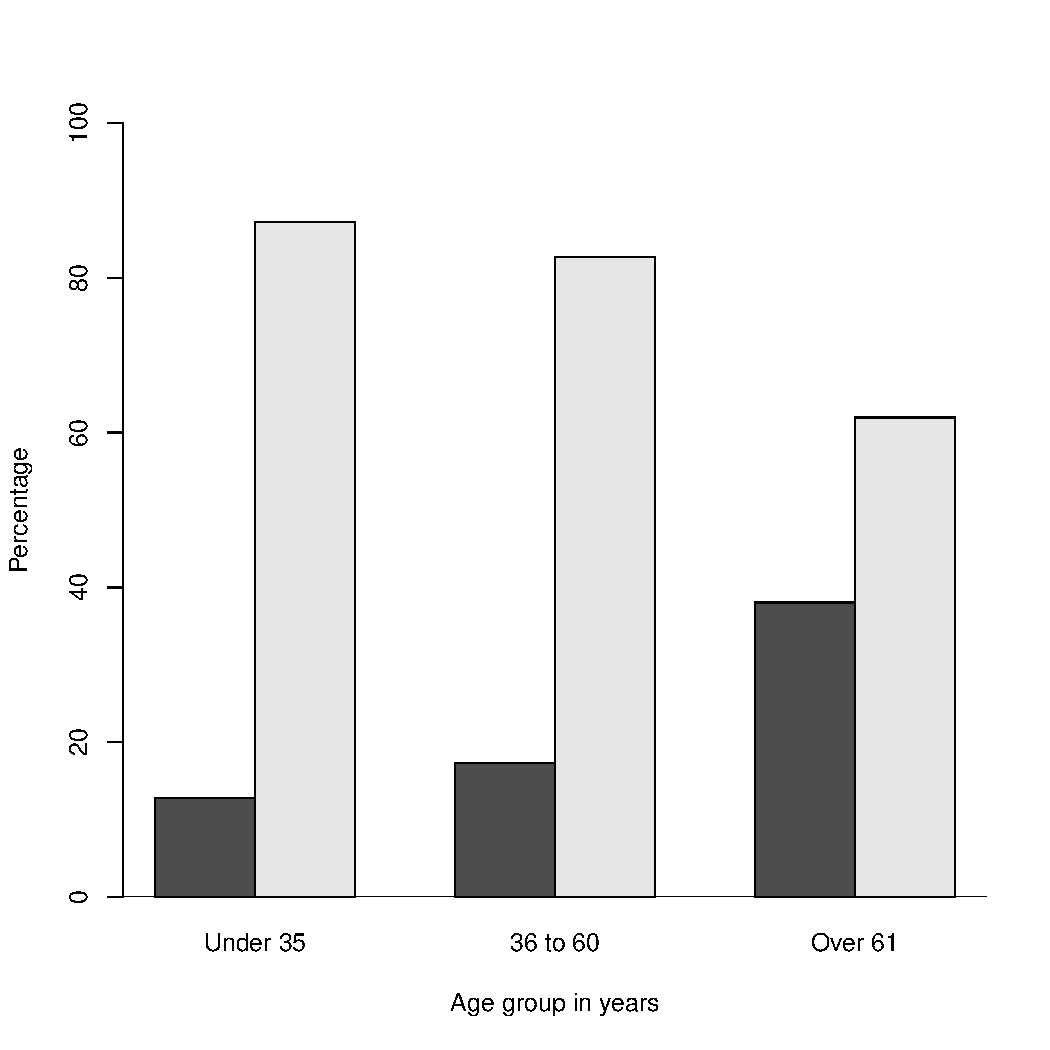
\includegraphics[width=0.45\linewidth]{figure/bar11-1} 

}



\end{knitrout}
\end{frame}

\begin{frame}[fragile]
  \frametitle{Adding space between bars}
\begin{knitrout}
\definecolor{shadecolor}{rgb}{0.965, 0.965, 0.965}\color{fgcolor}\begin{kframe}
\begin{alltt}
\hlkwd{barplot}\hlstd{(q5.age,} \hlkwc{beside} \hlstd{=} \hlnum{TRUE}\hlstd{,} \hlkwc{ylab} \hlstd{=} \hlstr{"Percentage"}\hlstd{,}
        \hlkwc{xlab} \hlstd{=} \hlstr{"Age group in years"}\hlstd{,} \hlkwc{ylim} \hlstd{=} \hlkwd{c}\hlstd{(}\hlnum{0}\hlstd{,} \hlnum{100}\hlstd{),}
        \hlkwc{space} \hlstd{=} \hlkwd{c}\hlstd{(}\hlnum{0.2}\hlstd{,} \hlnum{1.5}\hlstd{))}
\hlkwd{abline}\hlstd{(}\hlkwc{h} \hlstd{=} \hlnum{0}\hlstd{)}
\end{alltt}
\end{kframe}

{\centering 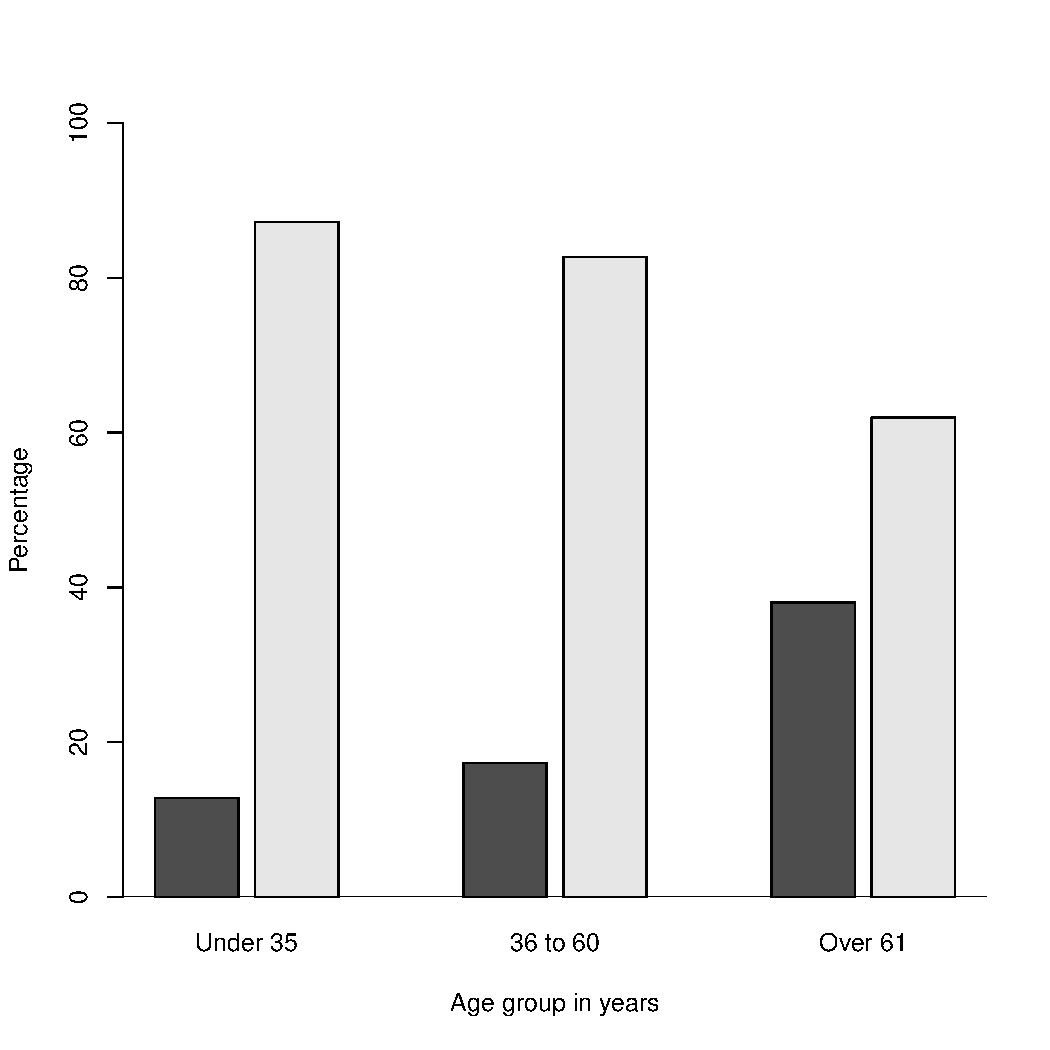
\includegraphics[width=0.45\linewidth]{figure/bar3-1} 

}



\end{knitrout}
\end{frame}

\begin{frame}[fragile]
  \frametitle{Shading with lines?}
\begin{knitrout}
\definecolor{shadecolor}{rgb}{0.965, 0.965, 0.965}\color{fgcolor}\begin{kframe}
\begin{alltt}
\hlkwd{barplot}\hlstd{(q5.age,} \hlkwc{beside} \hlstd{=} \hlnum{TRUE}\hlstd{,} \hlkwc{ylab} \hlstd{=} \hlstr{"Percentage"}\hlstd{,}
        \hlkwc{xlab} \hlstd{=} \hlstr{"Age group in years"}\hlstd{,} \hlkwc{ylim} \hlstd{=} \hlkwd{c}\hlstd{(}\hlnum{0}\hlstd{,} \hlnum{100}\hlstd{),}
        \hlkwc{space} \hlstd{=} \hlkwd{c}\hlstd{(}\hlnum{0.2}\hlstd{,} \hlnum{1.5}\hlstd{),} \hlkwc{density} \hlstd{=} \hlkwd{c}\hlstd{(}\hlnum{0}\hlstd{,} \hlnum{10}\hlstd{))}
\hlkwd{abline}\hlstd{(}\hlkwc{h} \hlstd{=} \hlnum{0}\hlstd{)}
\end{alltt}
\end{kframe}
\end{knitrout}
\vspace{-5mm}
\begin{knitrout}
\definecolor{shadecolor}{rgb}{0.965, 0.965, 0.965}\color{fgcolor}

{\centering 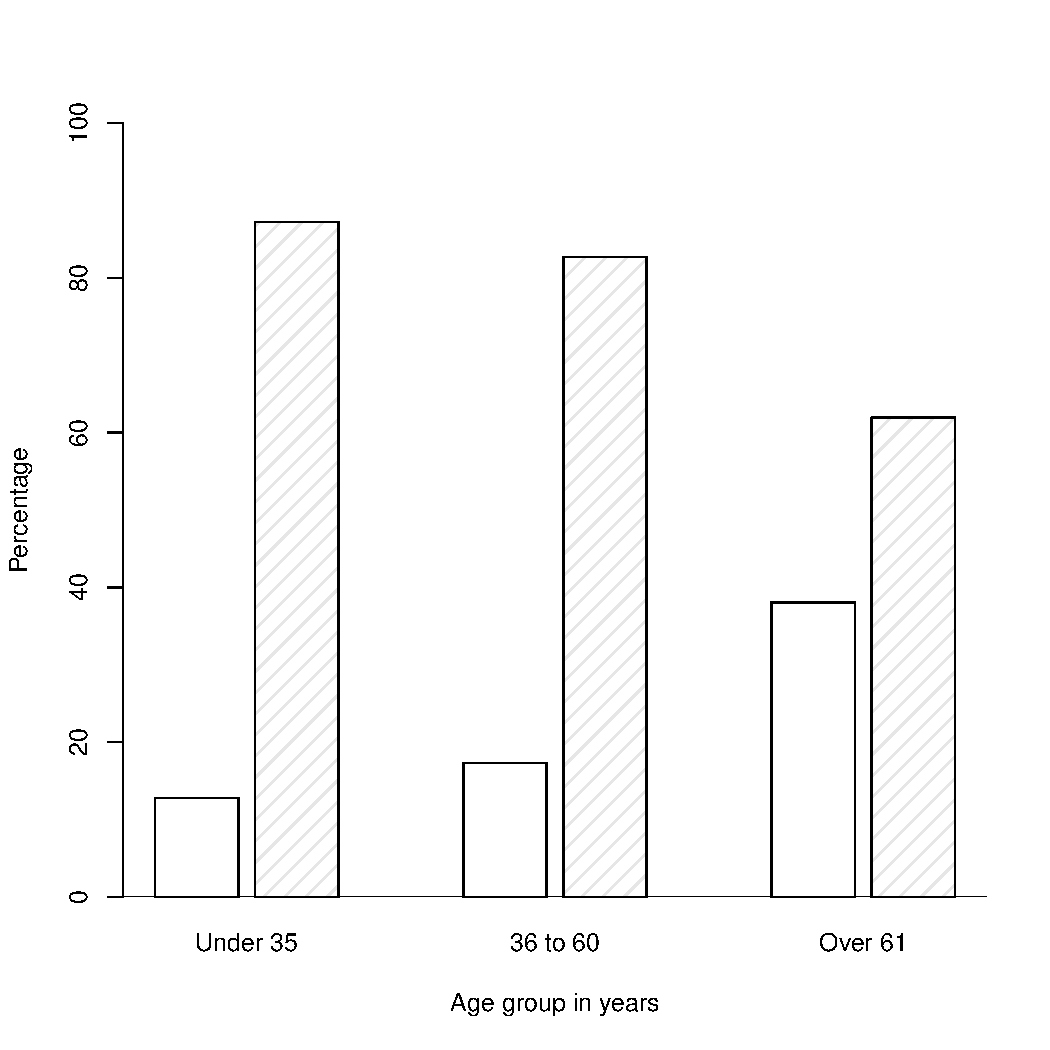
\includegraphics[width=0.4\linewidth]{figure/bar4-1} 

}



\end{knitrout}
\vspace{-3mm}
\begin{center}
  Can't see the shading?
\end{center}
\end{frame}

\begin{frame}[fragile]
  \frametitle{Shading with lines?}
The default colour for shading lines is pale white! Change to black using the \texttt{col} argument.
\begin{knitrout}
\definecolor{shadecolor}{rgb}{0.965, 0.965, 0.965}\color{fgcolor}\begin{kframe}
\begin{alltt}
\hlkwd{barplot}\hlstd{(q5.age,} \hlkwc{beside} \hlstd{=} \hlnum{TRUE}\hlstd{,} \hlkwc{ylab} \hlstd{=} \hlstr{"Percentage"}\hlstd{,}
        \hlkwc{xlab} \hlstd{=} \hlstr{"Age group in years"}\hlstd{,} \hlkwc{ylim} \hlstd{=} \hlkwd{c}\hlstd{(}\hlnum{0}\hlstd{,} \hlnum{100}\hlstd{),}
        \hlkwc{space} \hlstd{=} \hlkwd{c}\hlstd{(}\hlnum{0.2}\hlstd{,} \hlnum{1.5}\hlstd{),} \hlkwc{density} \hlstd{=} \hlkwd{c}\hlstd{(}\hlnum{0}\hlstd{,} \hlnum{10}\hlstd{),}
        \hlkwc{col} \hlstd{=} \hlstr{"black"}\hlstd{)}
\hlkwd{abline}\hlstd{(}\hlkwc{h} \hlstd{=} \hlnum{0}\hlstd{)}
\end{alltt}
\end{kframe}
\end{knitrout}
\end{frame}


\begin{frame}[fragile]
  \frametitle{Shading with lines?}
\begin{knitrout}
\definecolor{shadecolor}{rgb}{0.965, 0.965, 0.965}\color{fgcolor}

{\centering 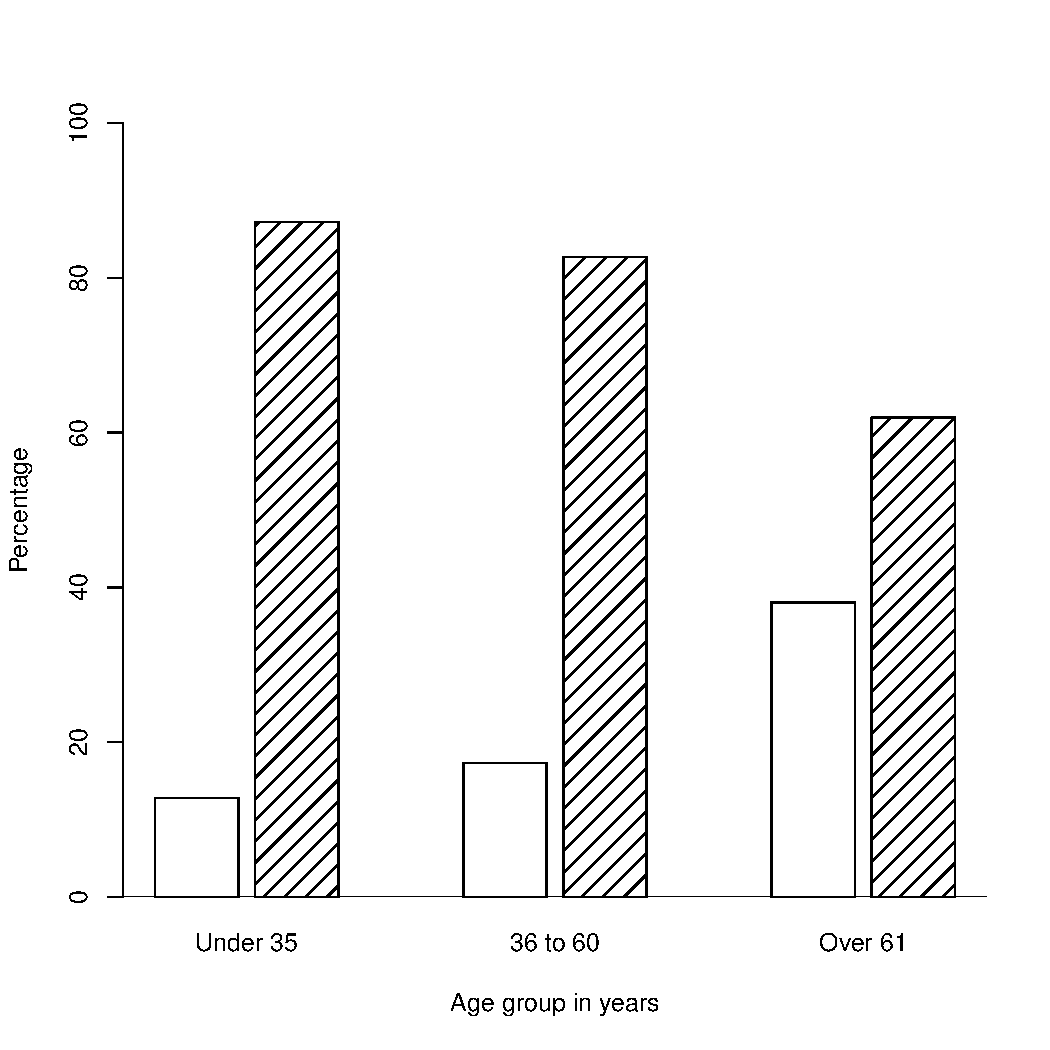
\includegraphics[width=0.6\linewidth]{figure/bar5-1} 

}



\end{knitrout}
\end{frame}


\begin{frame}[fragile]
  \frametitle{Color-filled bars?}
\begin{knitrout}
\definecolor{shadecolor}{rgb}{0.965, 0.965, 0.965}\color{fgcolor}\begin{kframe}
\begin{alltt}
\hlkwd{barplot}\hlstd{(q5.age,} \hlkwc{beside} \hlstd{=} \hlnum{TRUE}\hlstd{,} \hlkwc{ylab} \hlstd{=} \hlstr{"Percentage"}\hlstd{,}
        \hlkwc{xlab} \hlstd{=} \hlstr{"Age group in years"}\hlstd{,} \hlkwc{ylim} \hlstd{=} \hlkwd{c}\hlstd{(}\hlnum{0}\hlstd{,} \hlnum{100}\hlstd{),}
        \hlkwc{space} \hlstd{=} \hlkwd{c}\hlstd{(}\hlnum{0.2}\hlstd{,} \hlnum{1.5}\hlstd{),} \hlkwc{col} \hlstd{=} \hlkwd{c}\hlstd{(}\hlstr{"blue"}\hlstd{,} \hlstr{"green"}\hlstd{))}
\hlkwd{abline}\hlstd{(}\hlkwc{h} \hlstd{=} \hlnum{0}\hlstd{)}
\end{alltt}
\end{kframe}
\end{knitrout}
\end{frame}

\begin{frame}[fragile]
  \frametitle{Color-filled bars?}
\begin{knitrout}
\definecolor{shadecolor}{rgb}{0.965, 0.965, 0.965}\color{fgcolor}

{\centering 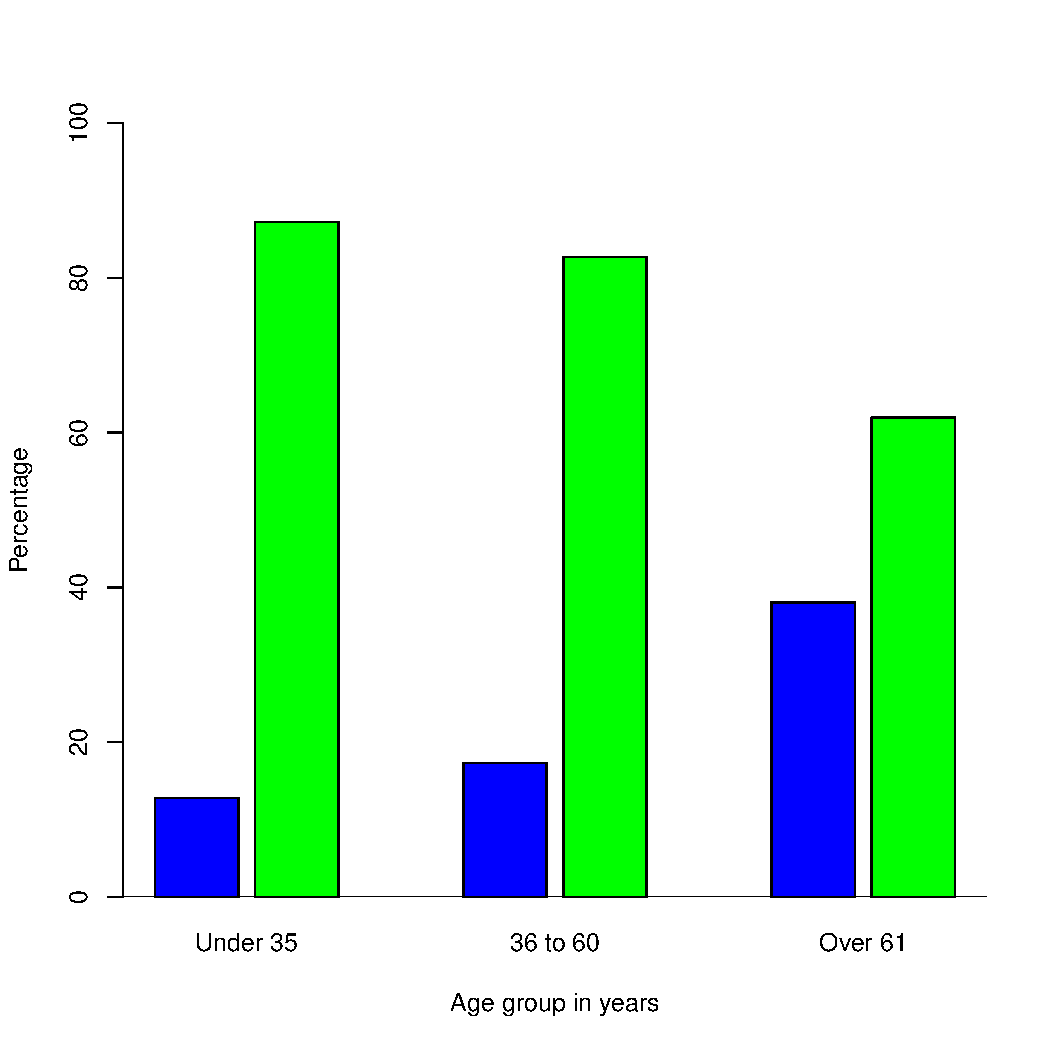
\includegraphics[width=0.6\linewidth]{figure/bar6-1} 

}



\end{knitrout}
\end{frame}

\begin{frame}[fragile]
  \frametitle{Legend?}
\begin{knitrout}
\definecolor{shadecolor}{rgb}{0.965, 0.965, 0.965}\color{fgcolor}\begin{kframe}
\begin{alltt}
\hlkwd{barplot}\hlstd{(q5.age,} \hlkwc{beside} \hlstd{=} \hlnum{TRUE}\hlstd{,} \hlkwc{ylab} \hlstd{=} \hlstr{"Percentage"}\hlstd{,}
        \hlkwc{xlab} \hlstd{=} \hlstr{"Age group in years"}\hlstd{,} \hlkwc{ylim} \hlstd{=} \hlkwd{c}\hlstd{(}\hlnum{0}\hlstd{,} \hlnum{100}\hlstd{),}
        \hlkwc{space} \hlstd{=} \hlkwd{c}\hlstd{(}\hlnum{0.2}\hlstd{,} \hlnum{1.5}\hlstd{),} \hlkwc{legend.text} \hlstd{=} \hlnum{TRUE}\hlstd{)}
\hlkwd{abline}\hlstd{(}\hlkwc{h} \hlstd{=} \hlnum{0}\hlstd{)}
\end{alltt}
\end{kframe}
\end{knitrout}
\end{frame}

\begin{frame}[fragile]
  \frametitle{Legend?}
\begin{knitrout}
\definecolor{shadecolor}{rgb}{0.965, 0.965, 0.965}\color{fgcolor}

{\centering 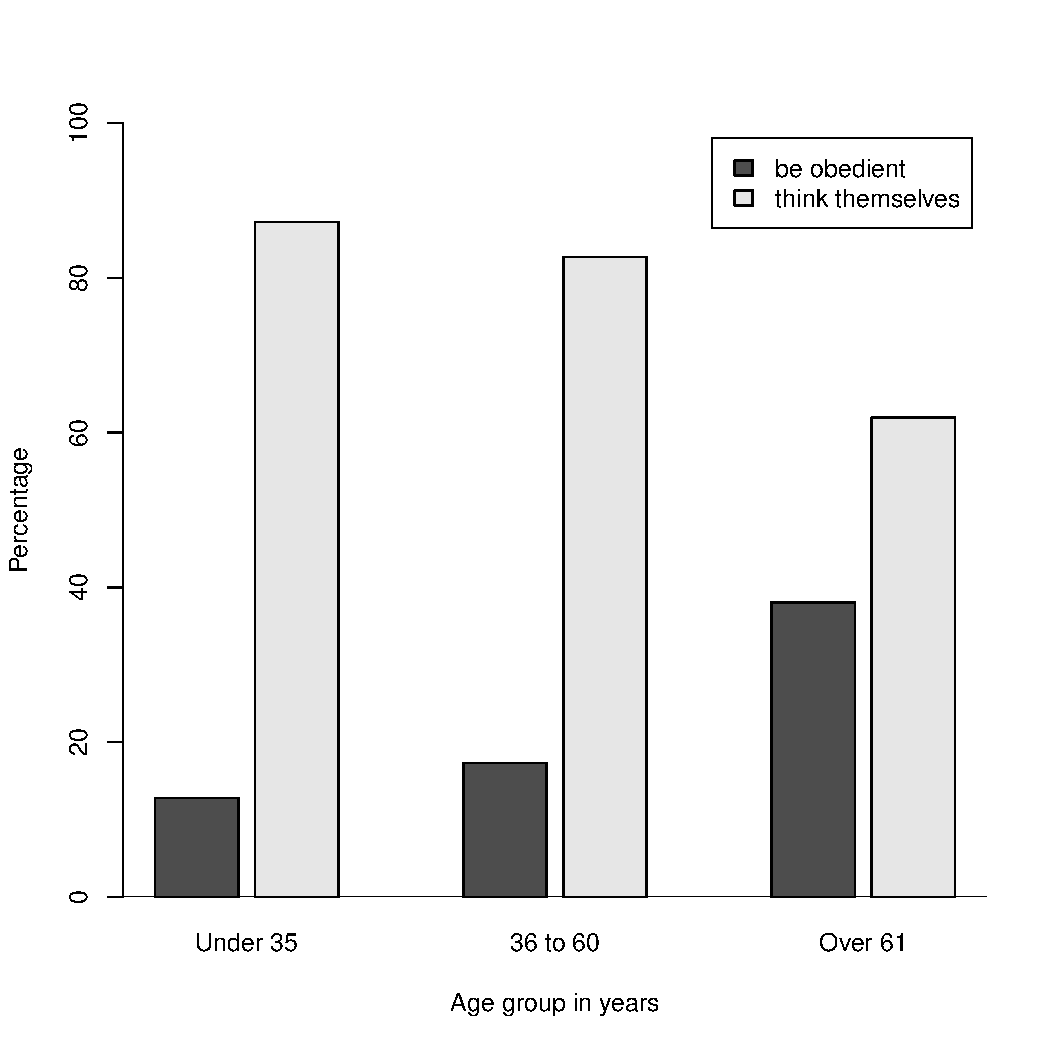
\includegraphics[width=0.6\linewidth]{figure/bar7-1} 

}



\end{knitrout}
\end{frame}
 


\begin{frame}[fragile]
  \frametitle{Further improvements}
\begin{itemize}
\item Larger title for axes
\item Get rid of the box drawn outside the legend
\item Larger legend
\end{itemize}
\begin{knitrout}
\definecolor{shadecolor}{rgb}{0.965, 0.965, 0.965}\color{fgcolor}\begin{kframe}
\begin{alltt}
\hlkwd{barplot}\hlstd{(q5.age,} \hlkwc{beside} \hlstd{=} \hlnum{TRUE}\hlstd{,} \hlkwc{ylab} \hlstd{=} \hlstr{"Percentage"}\hlstd{,}
        \hlkwc{xlab} \hlstd{=} \hlstr{"Age group in years"}\hlstd{,} \hlkwc{ylim} \hlstd{=} \hlkwd{c}\hlstd{(}\hlnum{0}\hlstd{,} \hlnum{100}\hlstd{),}
        \hlkwc{space} \hlstd{=} \hlkwd{c}\hlstd{(}\hlnum{0.2}\hlstd{,} \hlnum{1.5}\hlstd{),} \hlkwc{legend.text} \hlstd{=} \hlnum{TRUE}\hlstd{,}
        \hlkwc{args.legend} \hlstd{=} \hlkwd{list}\hlstd{(}\hlkwc{bty} \hlstd{=} \hlstr{"n"}\hlstd{,} \hlkwc{cex} \hlstd{=} \hlnum{1.3}\hlstd{))}
\hlkwd{abline}\hlstd{(}\hlkwc{h} \hlstd{=} \hlnum{0}\hlstd{)}
\end{alltt}
\end{kframe}
\end{knitrout}
\end{frame}


\begin{frame}[fragile]
  \frametitle{Further improvements}
\begin{knitrout}
\definecolor{shadecolor}{rgb}{0.965, 0.965, 0.965}\color{fgcolor}

{\centering 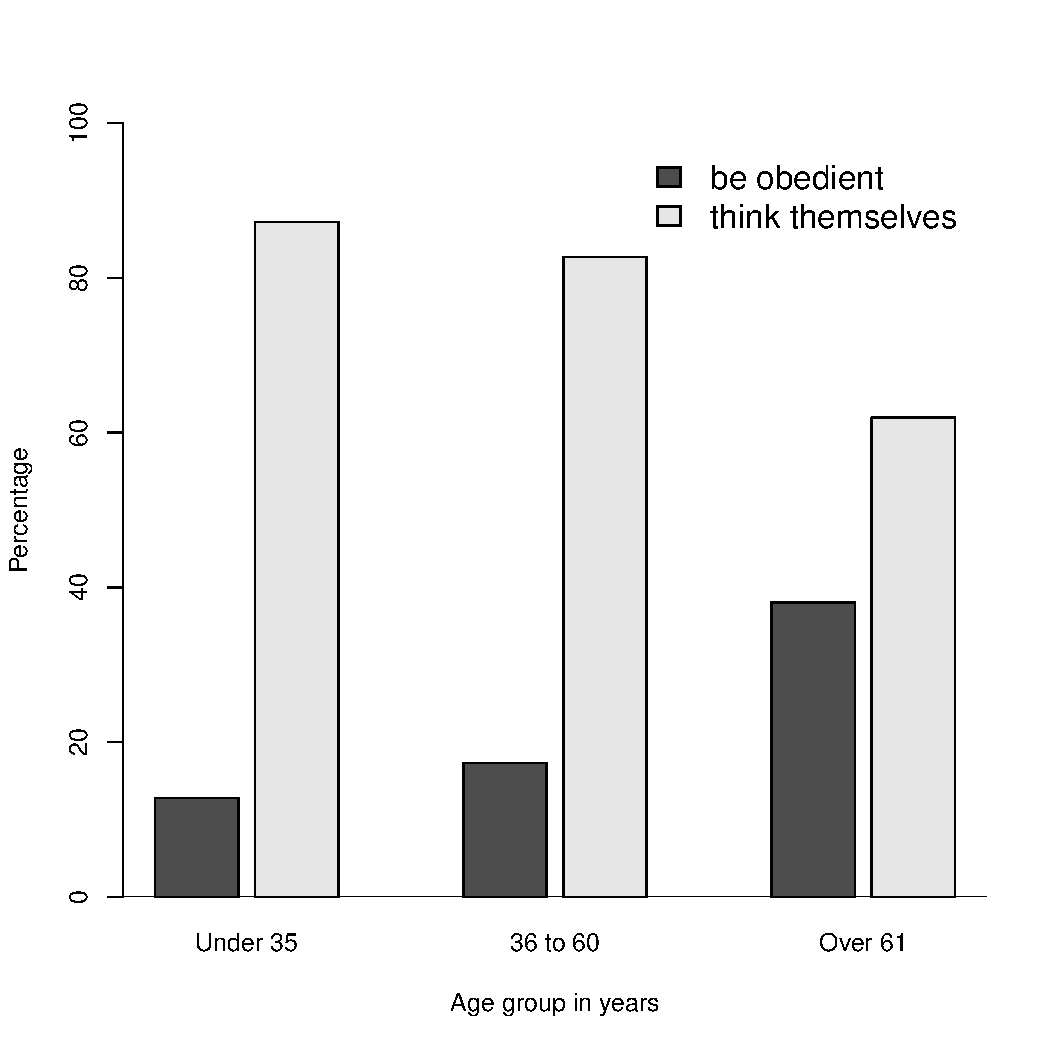
\includegraphics[width=0.6\linewidth]{figure/bar9-1} 

}



\end{knitrout}
\end{frame}


\begin{frame}[fragile]
  \frametitle{Histograms}
\begin{knitrout}
\definecolor{shadecolor}{rgb}{0.965, 0.965, 0.965}\color{fgcolor}\begin{kframe}
\begin{alltt}
\hlkwd{hist}\hlstd{(issp.df}\hlopt{$}\hlstd{Age)}
\end{alltt}
\end{kframe}

{\centering 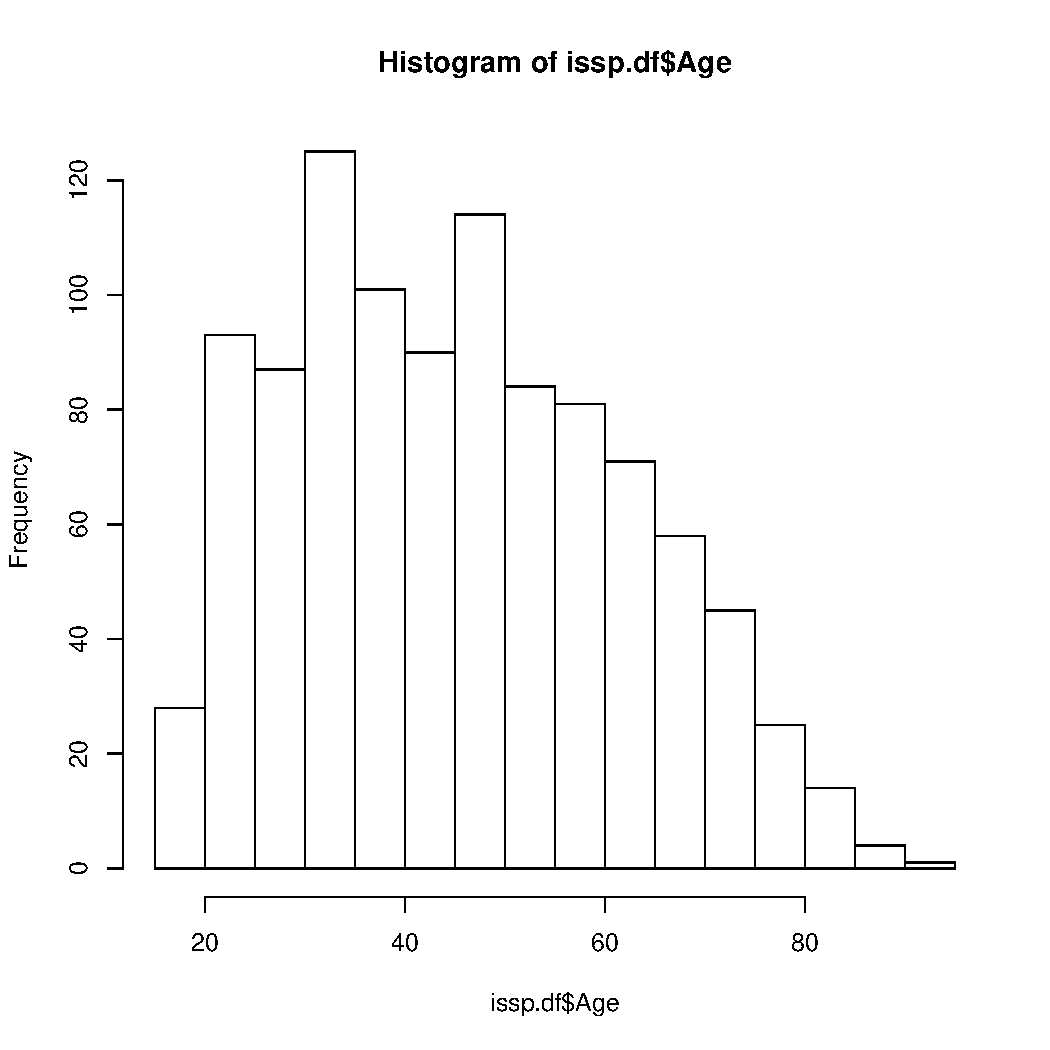
\includegraphics[width=0.6\linewidth]{figure/hist1-1} 

}



\end{knitrout}
\end{frame}

\begin{frame}[fragile]
  \frametitle{Fewer bins?}
\begin{knitrout}
\definecolor{shadecolor}{rgb}{0.965, 0.965, 0.965}\color{fgcolor}\begin{kframe}
\begin{alltt}
\hlkwd{hist}\hlstd{(issp.df}\hlopt{$}\hlstd{Age,} \hlkwc{breaks} \hlstd{=} \hlnum{10}\hlstd{)}
\end{alltt}
\end{kframe}

{\centering 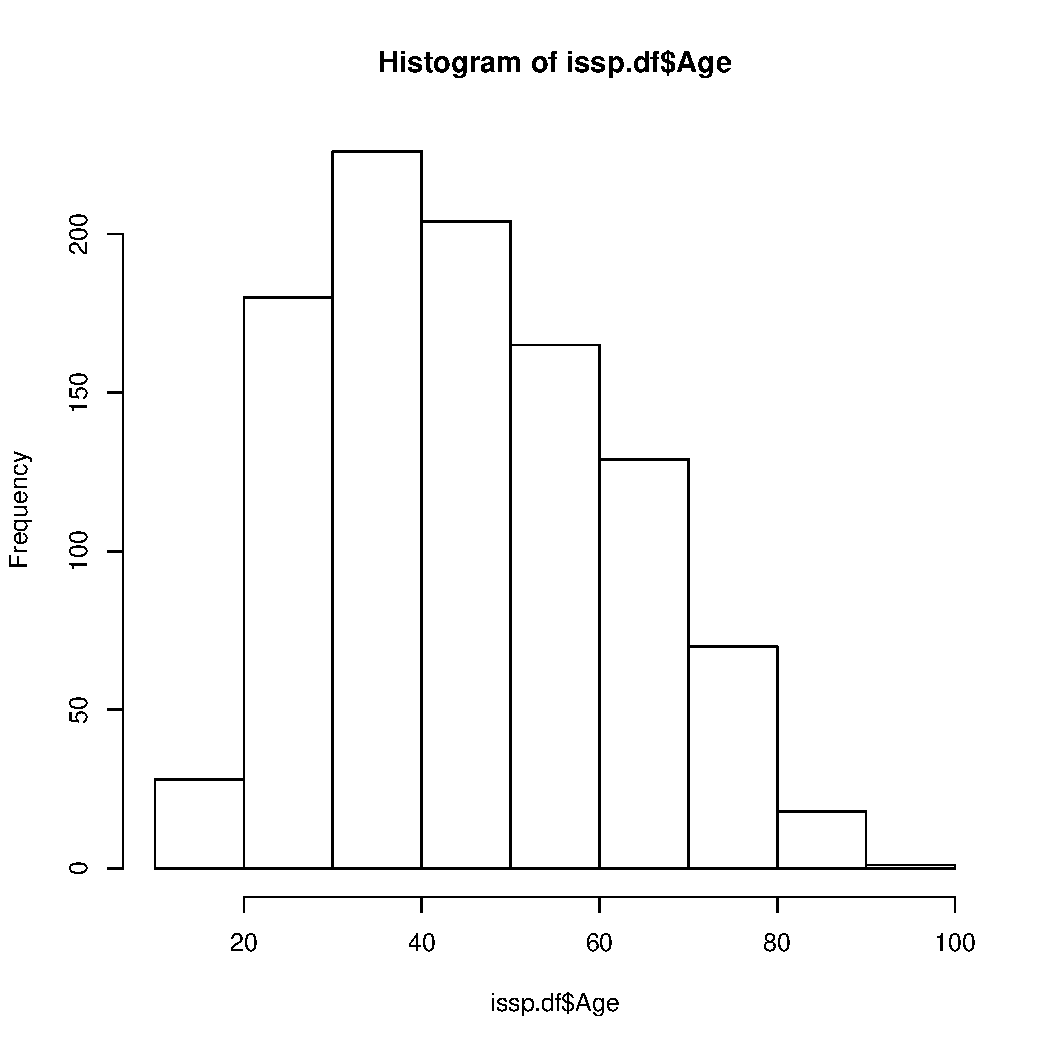
\includegraphics[width=0.6\linewidth]{figure/hist2-1} 

}



\end{knitrout}
\end{frame}


\begin{frame}[fragile]
  \frametitle{More bins?}
\begin{knitrout}
\definecolor{shadecolor}{rgb}{0.965, 0.965, 0.965}\color{fgcolor}\begin{kframe}
\begin{alltt}
\hlkwd{hist}\hlstd{(issp.df}\hlopt{$}\hlstd{Age,} \hlkwc{breaks} \hlstd{=} \hlnum{40}\hlstd{)}
\end{alltt}
\end{kframe}

{\centering 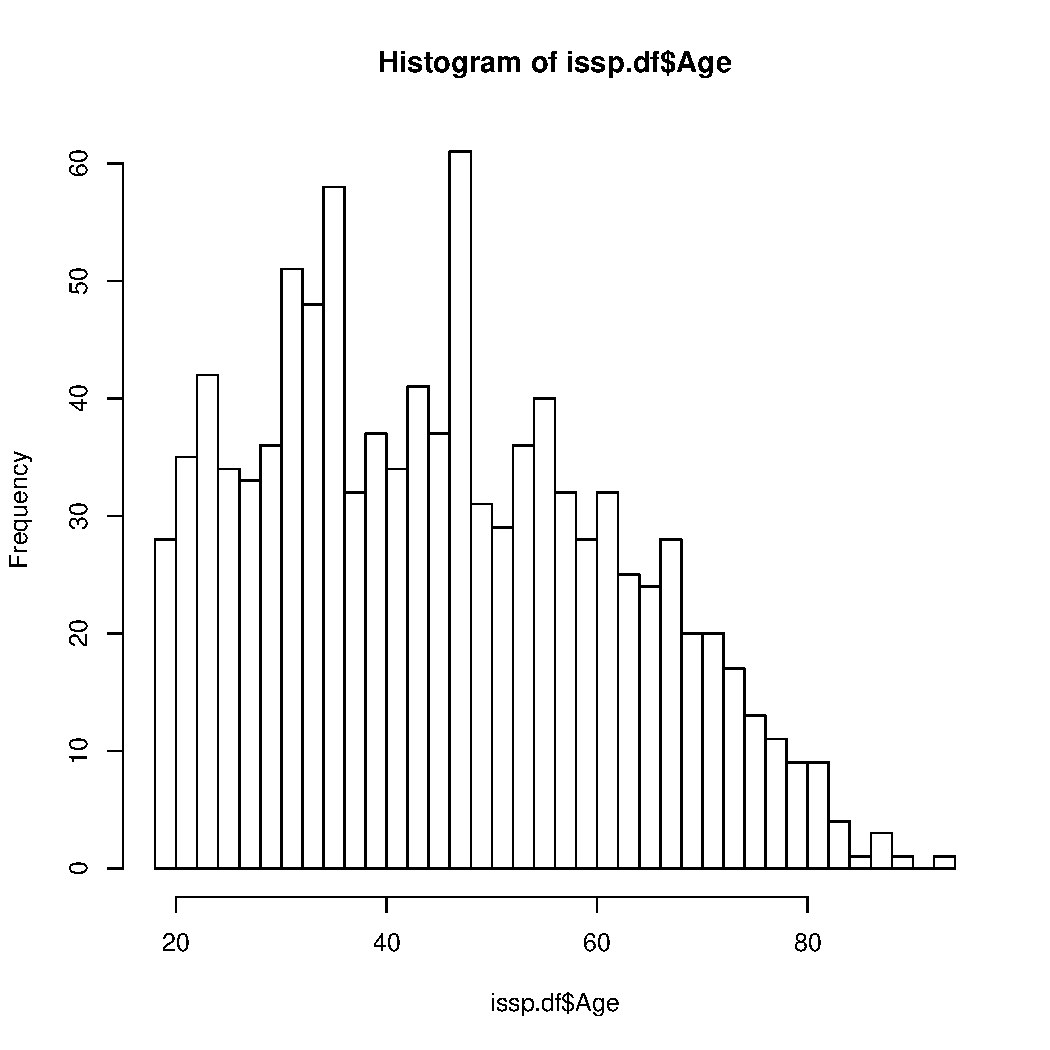
\includegraphics[width=0.6\linewidth]{figure/hist3-1} 

}



\end{knitrout}
\end{frame}


\begin{frame}[fragile]
  \frametitle{Always use meaningful axis labels}
\begin{knitrout}
\definecolor{shadecolor}{rgb}{0.965, 0.965, 0.965}\color{fgcolor}\begin{kframe}
\begin{alltt}
\hlkwd{hist}\hlstd{(issp.df}\hlopt{$}\hlstd{Age,} \hlkwc{xlab} \hlstd{=} \hlstr{"Age"}\hlstd{,} \hlkwc{main} \hlstd{=} \hlkwa{NULL}\hlstd{)}
\hlkwd{box}\hlstd{(}\hlkwc{bty}\hlstd{=}\hlstr{"l"}\hlstd{)}
\end{alltt}
\end{kframe}

{\centering 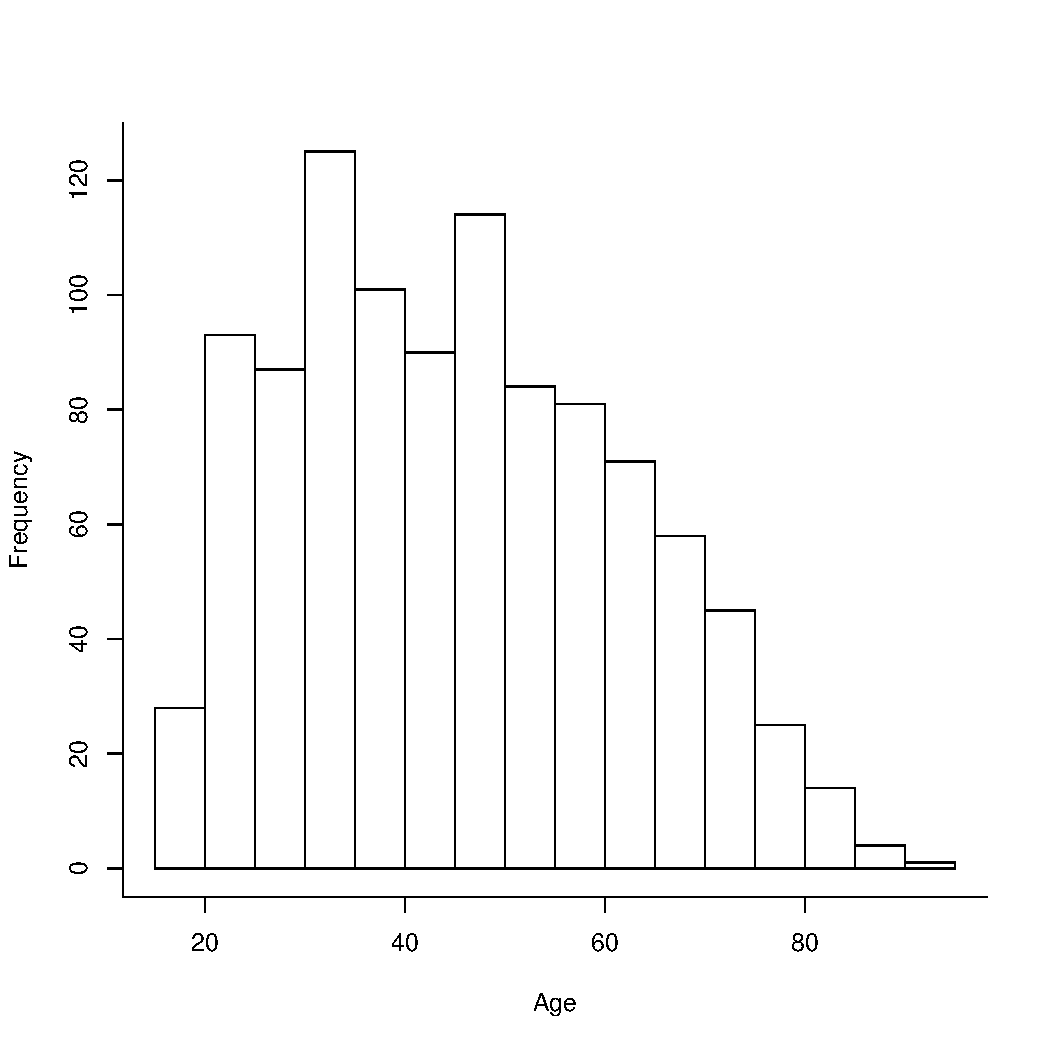
\includegraphics[width=0.5\linewidth]{figure/hist4-1} 

}



\end{knitrout}
\end{frame}

\begin{frame}[fragile]
\frametitle{Scatter plots}
\begin{itemize}
\item Not often used in the social sciences??
\item Introduced briefly here.
\item Used to display paired quantitative (numeric) data, e.g. age and score per respondent.
\item Make sure they are numeric.
\item Use \texttt{plot()} function, e.g.
\begin{knitrout}
\definecolor{shadecolor}{rgb}{0.965, 0.965, 0.965}\color{fgcolor}\begin{kframe}
\begin{alltt}
\hlkwd{with}\hlstd{(issp.df,} \hlkwd{plot}\hlstd{(Age, total.lik))}
\end{alltt}
\end{kframe}
\end{knitrout}
\end{itemize}
\end{frame}

\begin{frame}[fragile]
  \frametitle{Scatter plots}
\begin{knitrout}
\definecolor{shadecolor}{rgb}{0.965, 0.965, 0.965}\color{fgcolor}

{\centering 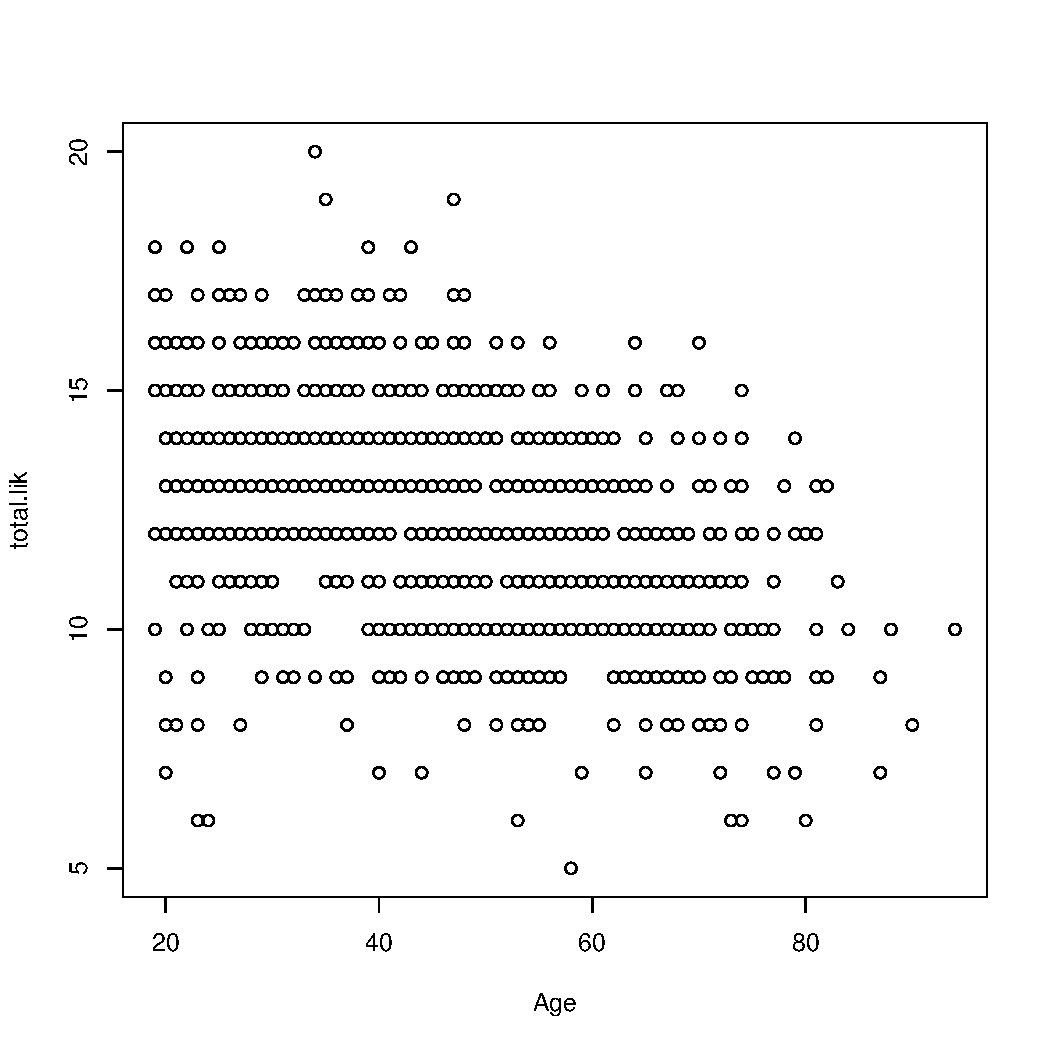
\includegraphics[width=0.6\linewidth]{figure/scat1-1} 

}



\end{knitrout}
\end{frame}

\begin{frame}[fragile]
  \frametitle{Graphical Parameters}
\begin{knitrout}
\definecolor{shadecolor}{rgb}{0.965, 0.965, 0.965}\color{fgcolor}\begin{kframe}
\begin{alltt}
\hlopt{?}\hlstd{par}
\hlstd{op} \hlkwb{<-} \hlkwd{par}\hlstd{(}\hlkwc{mfrow} \hlstd{=} \hlkwd{c}\hlstd{(}\hlnum{2}\hlstd{,} \hlnum{2}\hlstd{))}
  \hlkwd{with}\hlstd{(issp.df,} \hlkwd{boxplot}\hlstd{(total.lik}\hlopt{~}\hlstd{age.group,}
      \hlkwc{xlab} \hlstd{=} \hlstr{"Age Group"}\hlstd{,} \hlkwc{ylab} \hlstd{=} \hlstr{"Total score"}\hlstd{))}
  \hlkwd{barplot}\hlstd{(q5.age,} \hlkwc{beside} \hlstd{=} \hlnum{TRUE}\hlstd{,} \hlkwc{ylab} \hlstd{=} \hlstr{"Percentage"}\hlstd{,}
      \hlkwc{xlab} \hlstd{=} \hlstr{"Age group in years"}\hlstd{,} \hlkwc{ylim} \hlstd{=} \hlkwd{c}\hlstd{(}\hlnum{0}\hlstd{,} \hlnum{100}\hlstd{),}
      \hlkwc{space} \hlstd{=} \hlkwd{c}\hlstd{(}\hlnum{0.2}\hlstd{,} \hlnum{1.5}\hlstd{),} \hlkwc{legend.text} \hlstd{=} \hlnum{TRUE}\hlstd{)}
      \hlkwd{abline}\hlstd{(}\hlkwc{h} \hlstd{=} \hlnum{0}\hlstd{)}
  \hlkwd{hist}\hlstd{(issp.df}\hlopt{$}\hlstd{Age)}
  \hlkwd{with}\hlstd{(issp.df,} \hlkwd{plot}\hlstd{(Age, total.lik))}
\hlcom{## At end of plotting, reset to previous settings:}
\hlkwd{par}\hlstd{(op)}
\end{alltt}
\end{kframe}
\end{knitrout}
\end{frame}

\begin{frame}[fragile]
  \frametitle{Graphical Parameters}
\begin{knitrout}
\definecolor{shadecolor}{rgb}{0.965, 0.965, 0.965}\color{fgcolor}

{\centering 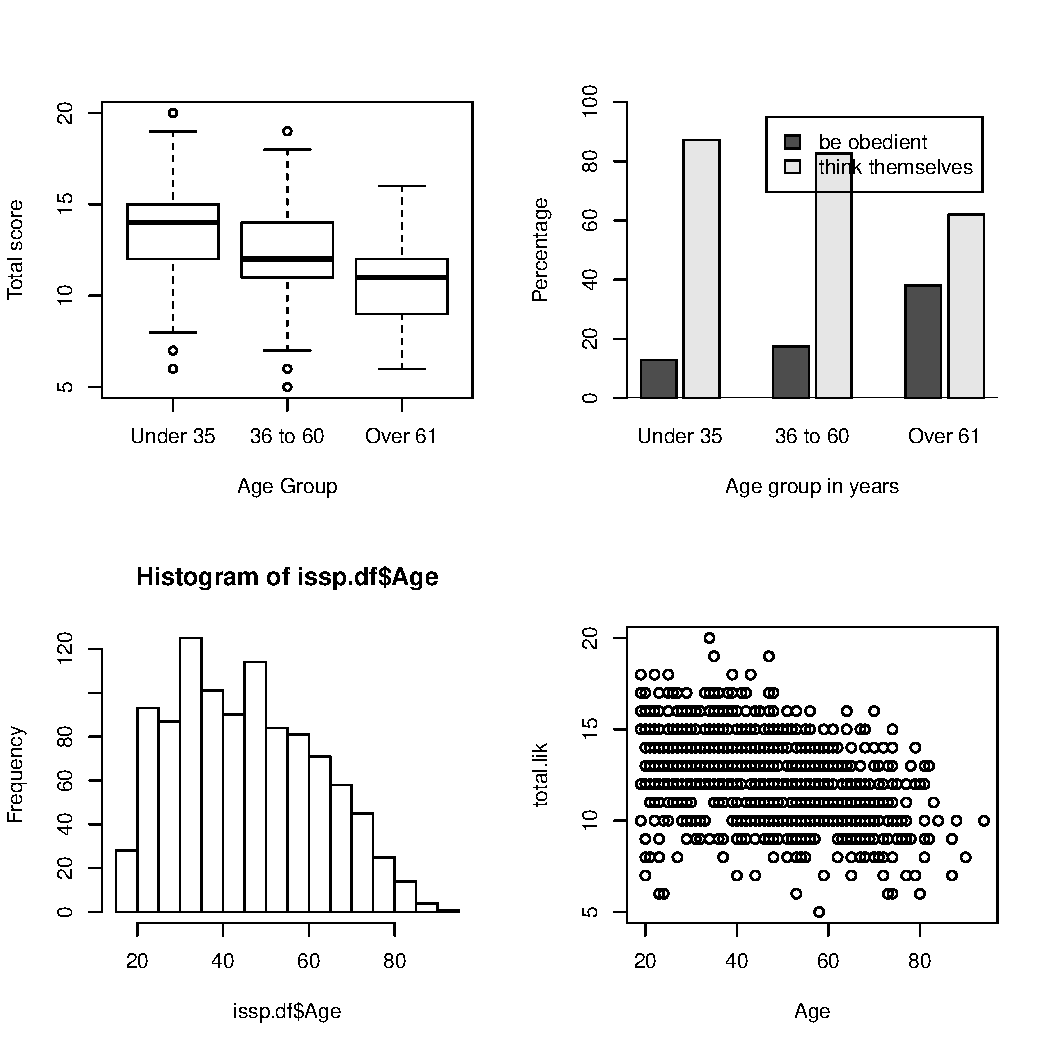
\includegraphics[width=0.6\linewidth]{figure/par1-1} 

}



\end{knitrout}
\end{frame}


\begin{frame}[fragile]
  \frametitle{Summary}
  \begin{itemize}
  \item Boxplots
  \item Histograms/Barplots
  \item Scatterplots
  \end{itemize}
\end{frame}

\end{document}
